\documentclass[conference]{IEEEtran}
\IEEEoverridecommandlockouts
% The preceding line is only needed to identify funding in the first footnote. If that is unneeded, please comment it out.
\usepackage{cite}
\usepackage{amsmath,amssymb,amsfonts}
%\usepackage{algorithmicx}
\usepackage{graphicx}
\usepackage{syntax}
\usepackage{textcomp}
\usepackage{xcolor}
\usepackage[numbers]{natbib} 
\usepackage{algorithm}
\usepackage{algpseudocode}
\usepackage{multirow}
\usepackage{pifont}
%\usepackage{subcaption}
\usepackage{subfigure}
\newcommand{\cmark}{\ding{51}}%
\newcommand{\xmark}{\ding{55}}%
\def\BibTeX{{\rm B\kern-.05em{\sc i\kern-.025em b}\kern-.08em
    T\kern-.1667em\lower.7ex\hbox{E}\kern-.125emX}}


%switch case statement
\newcommand{\SWITCH}[1]{\STATE \textbf{switch} (#1)}
\newcommand{\ENDSWITCH}{\STATE \textbf{end switch}}
\newcommand{\CASE}[1]{\STATE \textbf{case} #1\textbf{:} \begin{ALC@g}}
	\newcommand{\ENDCASE}{\end{ALC@g}}
\newcommand{\CASELINE}[1]{\STATE \textbf{case} #1\textbf{:} }
\newcommand{\DEFAULT}{\STATE \textbf{default:} \begin{ALC@g}}
	\newcommand{\ENDDEFAULT}{\end{ALC@g}}
\newcommand{\DEFAULTLINE}[1]{\STATE \textbf{default:} }
%switch case statement
\let\footnotesize\scriptsize

\algnewcommand{\LineComment}[1]{\State \(\triangleright\) #1}
\algdef{SE}[DOWHILE]{Do}{doWhile}{\algorithmicdo}[1]{\algorithmicwhile\ #1}%


\usepackage{expl3}
\ExplSyntaxOn
\newcommand\latinabbrev[1]{
	\peek_meaning:NTF . {% Same as \@ifnextchar
		#1\@}%
	{ \peek_catcode:NTF a {% Check whether next char has same catcode as \'a, i.e., is a letter
			#1., \@ }%
		{#1., \@}}}
\ExplSyntaxOff

\begin{document}

\title{Improved Bug Localization using Association Mapping and Information Retrieval\\
%{\footnotesize \textsuperscript{*}Note: Sub-titles are not captured in Xplore and
%/should not be used}
%\thanks{Identify applicable funding agency here. If none, delete this.}
}

%\author{\IEEEauthorblockN{Shamima Yeasmin~~~Mohammad Masudur Rahman~~~Chanchal K. Roy~~~ Kevin A. Schneider}
%\IEEEauthorblockA{\textit{Department of Computer Science} \\
%\textit{ University of Saskatchewan}\\
%Saskatoon, Canada \\
%shy942@mail.usask.ca, \{masud.rahman, chanchal.roy, kevin.schneider\}@usask.ca}
%\and
%\IEEEauthorblockN{Mohammad Masudur Rahman}
%\IEEEauthorblockA{\textit{dept. name of organization (of Aff.)} \\
%\textit{name of organization (of Aff.)}\\
%City, Country \\
%email address}
%\and
%\IEEEauthorblockN{Chanchal K. roy}
%\IEEEauthorblockA{\textit{dept. name of organization (of Aff.)} \\
%\textit{name of organization (of Aff.)}\\
%City, Country \\
%email address}
%\and
%\IEEEauthorblockN{Kevin A. Schneider}
%\IEEEauthorblockA{\textit{dept. name of organization (of Aff.)} \\
%\textit{name of organization (of Aff.)}\\
%City, Country \\
%email address}

%}

\maketitle

\begin{abstract}
Bug localization is one of the most challenging tasks undertaken by the developers during software maintenance.
Most of the existing studies rely on lexical similarity between the bug reports and source code for bug localization.
Unfortunately, such similarity always does not exist, and these studies suffer from vocabulary mismatch issues.
In this paper, we propose a bug localization technique that (1) not only uses lexical similarity between a given bug report and source code documents  
but also (2) exploits the association between keywords from the previously resolved bug reports and their corresponding changed source documents.
Experiments using a collection of 3,431 bug reports show that on average our technique can locate buggy files with a Top-10 accuracy of 74.06\%, a mean reciprocal rank@10 of 0.52 and a mean average precision@10 of 41\% which are highly promising. 
Comparison with the state-of-the-art techniques
and their variants report that our technique can improve upon them by 32.26\% in MAP@10 and 26.74\% in Top-5 accuracy. 
\end{abstract}

\begin{IEEEkeywords}
bug localization, bug report, source code, information retrieval, keyword-source code association
\end{IEEEkeywords}

\section{Introduction}
Bug localization is a process of locating such source code that needs to be changed in order to fix a given bug. 
Manually locating buggy files is not only time-consuming but also prohibitively costly in terms of development efforts \cite{Wang}. This is even more challenging for the large software systems. Thus, effective, automated approaches are highly warranted for localizing the software bugs. 
Traditional Information Retrieval (IR) based bug localization techniques \cite{Saha,Jian} accept a bug report and a subject system as inputs and then return a list of buggy entities (e.g., classes, methods) against the bug report. They localize the bugs by simply relying on the \emph{lexical similarity} between a bug report and the source code. 
Hence, they are likely to be affected by the quality and content of a submitted query (i.e., bug report). That is, if a query does not contain adequate information, then the retrieved results might not be relevant at all. As existing findings \cite{parninireval,fse2018masud} suggest, bug reports could be of low quality and could miss the appropriate keywords. 
 Thus, lexical similarity alone might not be sufficient enough to solve the bug localization problem. 
%However, static bug localization technique has an advantage over dynamic technique, as it does not require any working subject system rather it can apply on any stage of a system. 
%In this work, we additionally consider an association between bug reports and their corresponding changed code extracted from commit logs for the bug localization.

%\citet{Jian} first propose BugLocator based on revised Vector Space Model (rVSM) that uses the lexical similarity between bug report texts and source code documents. \citet{Saha} capture the structures of both bug reports and source documents, and then apply structured information retrieval for bug localization. \citet{Moreno} consider structural similarity between stack traces in the bug report and the project document structures for bug localization. However, all of these studies share one common limitation.

%In existing studies, information retrieval techniques  \cite{Jian} \cite{Saha} \cite{Moreno} \cite{Anh} \cite{Lukins} are applied to automatically search for relevant buggy files based on a given bug report. 
%In case of Text Retrieval (TR) based approaches, \citet{Jian} propose BugLocator based on revised Vector Space Model (rVSM), which requires the information extracted from both the bug reports and the source codes.
%Due to the fuzzy nature of information retrieval, textually matching bug reports against source
%files may have to concede noise (i.e., less relevant but accidentally matched words). Therefore, by treating
%files as single units or favoring large files, this technique \cite{Jian} is more
%likely to be affected by the noise in large files.
%One of the issue associated with TR-based technique is treating source codes as flat text. 
%Here, exploiting the structure of source code can be an useful way to improve bug localization accuracy.
%So, \citet{Saha} present BLUiR, which retrieve structural information from code constructs.
%However, bug reports often contain stack-trace information, which may provide direct clues for possible faulty files. Most existing approaches directly treat the bug descriptions as plain texts and do not explicitly consider stack-trace information. Here, \citet{Moreno} combine both stack trace similarity and textual similarity to retrieve potential code elements. 
%To deal with two issues associated with source code structure and stack trace information, 
%\citet{Chu}  proposed  a technique that use segmentation i.e., divides each source code file into segments and use stack-trace analysis, which significantly improve the performance of BugLocator.
%LDA topic-based approaches \cite{Anh} \cite{Lukins} assume that the textual contents of a bug report and it's corresponding buggy source files share some technical aspects of the system.
%Therefore, they develop topic model that represents those technical aspects as topic. 
%However, existing bug localization approaches applied on small-scale data for evaluation so far.
%Besides the problem of small-scale evaluations, the performance of the existing bug localization methods can be further improved too. For example, using Latent Dirichlet Allocation (LDA), only buggy files for 22\% of Eclipse 3.1 bug reports are ranked in the top 10 [25]. 
%But, now it is an important research question to know how effective these approaches are for locating bugs in large-scale (i.e., big data).
%In the field of query processing
%\citet{Sisman}  proposed a method that examines the files retrieved for the initial query supplied by a user and then selects from these files only those additional terms that are in close proximity to the terms in the initial query. Their \cite{Sisman} experimental evaluation on two large software projects using more than 4,000 queries showed that the proposed approach leads to significant improvements for bug localization and outperforms the well-known QR methods
%in the literature.
%Most of these IR-based bug localization techniques simply rely on only lexical similarity for retrieving relevant documents from the codebase. Hence, the search queries constructed from a given bug report should contain keywords similar to the code terms. Unfortunately, bug reports could be of low quality and could miss the appropriate keywords. Besides, an appropriate query also warrants for domain expertise on the project from a developer, which can always not be guaranteed. 

In order to address the limitations with lexical similarity, several existing studies \cite{Maletic, MarcusMaletic,irmarcus} derive underlying semantics of a text document by employing Latent Semantic Analysis (LSA). \citeauthor{irmarcus} and colleagues adopt this technology in the context of concept location \cite{irmarcus,MarcusMaletic}, program comprehension \cite{Maletic} and traceability link recovery problems \cite{MarcusLSI}, and reported higher performance than traditional Vector Space Model (VSM) and probabilistic models.
Unfortunately, their approach suffers from a major limitation.
%They use this information to identify traceability links based on similarity measures. To automatically recover traceability links from system documentation to program source code, \citet{MarcusLSI} proposed a method using Latent Semantic Indexing (LSI), and their experiments suggest that this technique is promising than VSM, and other probabilistic IR methods.
%Second, when treating files as single units, they are affected by the noise of the large files. This issue also reduces the performance of the applicability of exploiting lexical similarity measure.
Latent Semantic Indexing (LSI) requires the use of a dimensionality reduction parameter that must be tuned for each document collection \cite{Kontostathis}.
The results returned by LSI can also be difficult to interpret, as
they are expressed using a numeric spatial representation.
Other related studies \cite{LukinsBL,Nguyen} adopt Latent Dirichlet Allocation (LDA) for bug localization. However, they are also subject to their hyper-parameters and could even be outperformed by simpler models (e.g., rVSM \cite{Jian}).   

%such complex models are often outperformed simple 
%\citet{LukinsBL} apply  to localize buggy files and methods. 
%They used 322 bugs across 25 versions of three projects (Eclipse, Mozilla and Rhino) for the evaluation.
%\citet{Nguyen} propose BugScout and customize the original LDA approach for software bug localization. However, existing study \cite{Jian} has reported, 
%Results on several large-scale datasets showed good performance.

\begin{table*}[t]
	\centering
	\caption{A working example of BLuAMIR}
	\label{tab:workingexample}
	\vspace{-.2cm}
	\resizebox{7.1in}{!}{%
		\begin{tabular}{c|l|c|c||l|c|c|c|c}
			\hline
			%\begin{tabular}[c]{@{}c@{}}\#Bugs for \\ developing \\ map databases\end{tabular} &
			& \multicolumn{3}{c||}{\textbf{VSM: Lexical Similarity Only}} &
			\multicolumn{5}{c}{\textbf{BLuAMIR: Lexical Similarity + Implicit Association}}\\
			\hline
			\textbf{Rank}
			& \textbf{Retrieved Documents } 
			&  \textbf{$\mathbf{Score_{VSM}}$}  & 
			\textbf{Ground Truth}  &
			\textbf{Retrieved Documents } &
			\textbf{$Score_{VSM}$}  & 
			\textbf{$Score_{Assoc}$} &
			\textbf{$Score_{Total}$} &
			
			\textbf{Ground Truth}\\
			\hline
			\hline
			1 &  WorkingSetLabelProvider.java  & 1.00  & \checkmark &WorkingSetLabelProvider.java & 0.60  & 0.25  & 0.85 & \checkmark \\
			\hline
			2 & ImageFactory.java  & 0.80  & \xmark & WorkingSet.java & 0.35 & 0.35 & 0.70 &  \checkmark \\ 
			\hline
			3 & WorkingSetMenuContributionItem.java &  0.76  & \xmark &IWorkingSet.java &0.45 &0.22 & 0.67 &  \checkmark\\
			\hline
			4 &  IWorkingSet.java &  0.75 & \checkmark & WorkingSetTypePage.java &0.38 & 0.25 & 0.63 &  \xmark\\
			\hline
			5 & ProjectImageRegistry.java  & 0.70  & \xmark & CommandImageService.java &0.30 &0.33 & 0.63 &  \xmark \\
			\hline
			%			& 0.68 & IWorkingSetManagerTest.java & \xmark &0.31 & 0.29 & 0.60 & WorkbenchImages.java & \checkmark\\
			%			\cline{2-9}
			%			& 0.67 & IWorkbenchPartDescriptor.java & \xmark & 0.33 & 0.27 & 0.60 & WorkingSetAdapterFactory.java & \checkmark \\
			%			\cline{2-9}
			%			& 0.65 & MockWorkingSetPage.java & \xmark  & 0.30 & 0.27 & 0.57 & EditorIconTest.java & \xmark\\
			%			\cline{2-9}
			%			& 0.65 & MissingImageDescriptor.java & \xmark  &0.30 &0.27 & 0.57 & PerspectiveDescriptor.java & \xmark \\
			%			\cline{2-9}
			%			& 0.64 & WorkingSetTypePage.java & \xmark & 0.24 & 0.33 & 0.57 & IAction.java & \xmark\\
			
	\end{tabular}}
	\centering
\end{table*}
\begin{table}[!tb]
	\caption{A Bug Report (\#37026, eclipse.UI.platform)}
	\label{tab:BugInfo}
	\vspace{-.4cm}
	%\centering
	\begin{center}
		\begin{tabular}{ p{1.5cm} | p{6cm}}
			\hline
			\textbf{Field}  & \textbf{Content} \\
			\hline
			\hline
			Title & [Working Sets] IWorkingSet.getImage should be getImageDescriptor
			\\
			\hline
			Description &  
		build 20030422
		
		IWorkingSet.getImage returns an ImageDescriptor and should therefore be named 
		getImageDescriptor.
		This is new API in 2.1. Should consider deprecating getImage and creating 
		getImageDescriptor.\\
			\hline
		\end{tabular}
	\end{center}
	%\centering
\end{table}


In this paper, we propose a bug localization approach namely BLuAMIR that not only considers \emph{lexical similarity} between a bug report (the query) and the source code but also captures \emph{implicit association} between them from the bug fixing history. First, we determine the lexical similarity between each source document and the query using Vector Space Model (VSM).
Second, we construct association maps between keywords of previously fixed bug reports and their corresponding changed documents using a bipartite graph. Third, we prioritize such source documents that are associated with the keywords (from query at hand) in these maps. Then, we rank the source documents based on their \emph{lexical} and \emph{association scores}.
Thus, our approach caters for the vocabulary mismatch between a bug report (the query) and the source code with implicit association. 
That is, unlike traditional IR-based approaches \cite{Jian,Saha}, it could return the buggy documents even if the query does not lexically match with the source code documents. Our approach also does not require the dimensionality reduction since we use a finite graph rather than a large sparse term-document matrix \cite{MarcusLSI,MarcusMaletic}.



%using a keyword-source association constructed from fixed bug information. 
%Our proposed technique also overcomes the issue with large files. Lexical similarity based approaches often suffer from the noise in the large documents during relevance estimation. Construction of association mapping between large source documents and an query does not require any direct vocabulary matching. Thus, our approach is not affected by the noise from large source documents and can rank the documents more effectively.
%The vocabulary between keywords extracted from a previously fixed bug report and its corresponding source code can not be matched, but can be linked in an association mapping. Thus, by exploiting this kind of relationship can aid locating future bug even if there exist no matched keywords between keywords from that bug and recommended source code.
%We compare the performance of our proposed tool with a state of the art bug localization techniques \cite{Jian}.

We evaluate our technique in three different aspects using
three widely used performance metrics and 3,431 bug reports (i.e.,
queries) from four open source subject systems. 
First, we evaluate in terms of the performance metrics, and contrast with two replicated baselines -- Latent Semantic Indexing (LSI) \cite{MarcusLSI} and basic Vector Space Model (VSM) \cite{vector-space-model}.
BLuAMIR localizes bugs with 9\%--37\% higher accuracy (i.e., Hit@10), 12\%--63\% higher precision (i.e., MAP), and 11\%--64\% higher reciprocal ranks (i.e., MRR) than these baselines (Sections \ref{RQ4answer}, \ref{RQ1answer}).
%BLuAMIR also localizes bugs with in average 9\% higher accuracy (i.e.,
%Hit@10), 12\% higher precision (i.e., MAP@10) and 11\%
%higher result ranks (i.e., MRR@10) than the replicated baseline VSM (Section \ref{RQ1answer}).
%BLuAMIR localizes bugs with in avaerage 57\% higher accuracy (i.e., Hit@10), 81\% higher precision(i.e., MAP@10) and 94\% higher resul ranks(i.e., MRR@10) than replicated BugLocator \cite{Jian} (section \ref{RQ1answer}).
Second, we compare our technique with three state of the art approaches -- BugScout \cite{Nguyen}, BugLocator \cite{Jian} and BLUiR \cite{Saha} (Section \ref{RQ4answer}).
Our technique can localize bugs with 6\%--54\% higher accuracy (i.e., Hit@5), 4\%--32\% higher precision (i.e., MAP) and 8\%--27\% higher reciprocal ranks (i.e., MRR) than these state-of-the-art approaches.
%with 58.79\% higher accuracy at Hit@1, 54.01\% higher accuracy at Hit@5 and 49.11\% higher accuracy at Hit@10 than BugScout \cite{Nguyen}.
%BLuAMIR performs 26.74\% higher accuracy at Hit@5, 32.26\% higher precision (i.e., MAP@10) and 26.83\% higher result ranks (i.e., MRR@10) than BugLocator \cite{Jian}.
%Our technique also shows 5.63\% higher accuracy at Hit@5, 4\% higher precision (i.e., MAP@10) and 7.79\% higher recall rate (i.e., MRR@10) than BLUiR \cite{Saha}.
%12\% in MAP@10
%and 12.6\% in Top-5 accuracy over the state-of-the-art (Section \ref{RQ4answer}).
Third, in terms of query-wise improvement, BLuAMIR improves result ranks of 41\% more and degrades 19\% less queries than baseline VSM (Section \ref{answerRQ3}) with Eclipse system.

Thus, this paper makes the following contributions:
\begin{itemize}
	\item A novel technique that not only considers the lexical similarity between a bug report and the source code but also exploits their implicit associations through bug-fixing history for bug localization.
	\item Comprehensive evaluation of the technique using three widely used performance metrics and a total of 3,431 bug reports from four subject systems --Eclipse, SWT, AspectJ and ZXing.
	\item Comparison with not only two baselines \cite{vector-space-model,MarcusLSI} but also three state-of-the-art approaches -- BugScout \cite{Nguyen}, BugLocator \cite{Jian} and BLUiR \cite{Saha} with statistical tests.
	\item Experimental meta data and our used dataset for  replication and third party reuse.
\end{itemize}

The rest of the paper is organized as follows. Section \ref{sec:motivatingexample} discusses a motivating example of our proposed approach, and Section \ref{sec:proposedmethod} presents proposed bug localization method for BLuAMIR, and Section \ref{sec:expANDdiss} focuses on the conducted experiments and experimental results, and Section \ref{sec:threats} identifies the possible threats to validity, and Section \ref{relatedwork}
discusses the existing studies related to our research, and finally,  
Section \ref{sec:conclusionANDfuture} concludes the paper with future plan.
\section{Motivating Example}\label{sec:motivatingexample}
Let us consider a bug report (ID 37026) on the Eclipse UI Platform. Table \ref{tab:BugInfo} shows the \textit{title} and \textit{description} of the bug report. We preprocess both fields, and construct a query. Then we apply both Vector Space Model (VSM) and our approach on this query, and locate possible buggy files. 
%The retrieved ranked results are presented in Table \ref{tab:workingexample}. 
%From the commit log, it is found that gold set contains 14 number of source code for this bug. 
In Table \ref{tab:workingexample}, we can see that basic VSM approach locates only 2 buggy files in Top-5 where, our proposed tool BLuAMIR correctly identifies 3 buggy files. The ranking from basic VSM is 1 and 4 where the rank from BLuAMIR is 1,2,3. However, VSM and association scores are also provided for each recommended buggy file. 
Note that Same file is retrieved in rank 1 for both techniques. 
The buggy file,  
IWorkingSet.java was in the fourth position by VSM, but BLUAMIR returned it at the second position which is promising.

We also investigate why BLuAMIR can locate more buggy files than VSM.  
VSM score is based on overlap of terms found both in the bug reports and source files. On the contrary, association score do not directly compare terms between bug reports and source files. So vocabulary mismatch problem is resolved here. Moreover, in the working example, this association map aids locating more buggy files than VSM technique. IF we go deeper, we can find that due to vocabulary missmatch problem, VSM failed to retrieve some buggy files. Our proposed approach makes use of an association map that successfully captures previous relationship between bug report keywords and their source buggy files. 
In BLuAMIR, we collect keywords from a current bug report (i.e., query) and then retrieve their associated source files from the constructed association map. 
This association map is created from keywords extracted from previously fixed bug report and their fixed buggy codebase. So, the idea is, if a current bug shares same keywords (i.e., concepts) with a previous fixed bug, there is possibility they might share some codebase. This is how our proposed approach overcome vocabulary missmatch problem.

\begin{figure*}
	\centering
	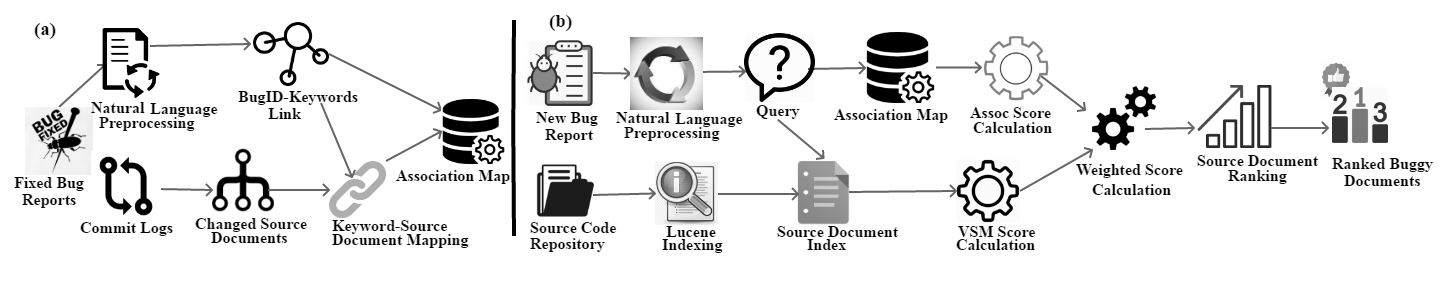
\includegraphics[scale=0.60]{SD-Feb04}
	\caption{Proposed Schematic Diagram: (a) Construction of association map between bug report keywords and source documents and (b) Bug Localization Using VSM and association score}
	\label{fig:systemDiagram}
\end{figure*}
\section{BLuAMIR: Proposed Approach for Bug Localization} \label{sec:proposedmethod} 
Figure \ref{fig:systemDiagram} shows the schematic diagram of our proposed approach.
%Our proposed approach combine lexical similarity and co-occurence similarity measure.  \citet{Jian} proposed BugLocator based on two different similarity scores- one is rVSM score and the other one is Simi score. 
First, we (a) construct an association map between the bug reports and their corresponding changed source documents with the help of bug-fixing history.
%where the inherent association between past bug reports and their changed documents are leveraged.
%In BLuAMIR, we follow two different approach for computing source code ranks.
Then we (b) retrieve buggy source code documents for a given query (bug report) by leveraging not only their lexical similarity but also their implicit associations derived from the association map above.   
%based on two different scores - VSM and association.  
%However, we have divided our approach into two different sections or parts- 1) calculate rVSM and Simi scores or VSM score and co-occurence measure and 2) combine all three or two scores in order to localize recommended buggy source files for a given newly reported bug. 
%As we have combined two existing scores with our proposed word co-occirence score, 
We discuss different parts of our proposed approach -- BLuAMIR -- in the following sections.

\subsection{Construction of Association Map}\label{sec:MapConstruction}
We construct an association map between keywords from previously fixed bug reports and their corresponding changed source documents.
The map construction involves three steps.
We not only show different steps of our map construction in Fig. \ref{fig:systemDiagram}-(a) but also provide the relevant pseudo-code in  Algorithm \ref{algo:map}. We discuss each of these steps as follows:

%refer to both figure and algorithm in the texts. 


\textbf{Keyword Extraction from Bug Reports:} First, we collect \emph{title} and \emph{description} of each bug report extracted from a subject system.  
Then we perform standard natural language preprocessing, and remove punctuation marks, stop words and small words from them. Stop words contain very little semantic for a sentence. Stemming extracts the root of each of the word. We use this stop word list\footnote{{1}https://www.ranks.nl/stopwords} during stop word removal and Porter Stemming stemmer\footnote{{2}http://tartarus.org/martin/PorterStemmer/} for stemming. Finally, we select a list of remaining keywords from each bug report. 
So, we create a mapping relationship between bug IDs and keywords contained in those bug reports, as described in Algorithm \ref{algo:map} line 5. We also construct another connected relationship between keywords and bug IDs, presented in
line 6 of Algorithm \ref{algo:map}.

% We then retrieve the source documents that were changed in order to fix each reported bug (i.e., bug report).
%which have been changed in order to fix a given bug. %Here the idea is, we first extract keywords from bug report and corresponding buggy source code files information for the same bug report from commit log. Then


%bug report keywords and the changed source documents.
%database by leveraging this connected relationship. 
%Mapping each keyword can be linked to one or more source code files according to commit logs. Similarly, each source code file can be linked to one or more keywords. 
%Algorithm \ref{algo:map} shows pseudo-code for the construction of our mapping database. 
%We divide this into three steps as follows.  
%This way we connect keywords and source code files to form an association map database named keyword-source code links. 

%This section can be further divided into several parts: keyword extraction from bug reports, source code information extraction from commit logs, keyword- source code linking. We also create an algorithm for creating association map database between bug report keywords into their buggy source files, which is given in Algorithm \ref{algo:map}. However, several steps of map database construction are discussed in the followings:

\begin{algorithm}[!t]
	\caption{Construction of Association Map}
	\label{algo:map}
	\begin{algorithmic}[1]
		\Procedure{MapConstruction}{$BRC$, $CommitLogs$}
		
		\LineComment{$BRC$: a collection of bug reports}
		
		\LineComment{$CommitLogs$: a collection of commit messages}
		\State $MAP_{KS} \gets$ \{\}
		\Comment{an empty association map}
		%\Comment{creating adjacency map database from the bug reports collection}
		%\State $MAP_{adj} \gets$ createAdjacencyDatabase($BRC$)
		%\Comment{creating a map that links keywords into their bug ids}
		\State $MAP_{bk} \gets$ createBugIDtoKeywordMap($BRC$)
		
		\Comment{Create Map between BugID and Keywords}
		
		\State $MAP_{kb} \gets$ createKeywordtoBugIDMap($MAP_{bk}$)
		
		\Comment{Create Map between Keywords and BugID}
		
		\State $MAP_{bs} \gets$ createBugIDtoSourceMap($CommitLogs$)
		
		\Comment{Create Map between BugID and codebase}
		
		\Comment{Linking keywords into change source code}
		%\LineComment{preprocess the collected keywords}
		%\For{Keyword $K_i \in$ $K$}
		\State $KB \gets$ collectKeywords($MAP_{kb}$)
		
		
		
		\For{keywords $KB_{_i}$ $\in$ $KB$}
		\State $BUG_{id} \gets$ retrieveBugIds ($KB_{_i}$)
		\For{each bug id $BUG_{id_j} \in BUG_{id}$}
		\State $SF_{link} \gets$ getLinkedSourceFiles($MAP_{bs}$, $BUG_{id}$)
		
		\Comment{Retrieve associated source from $MAP_{bs}}$
		%\State $MAO_{BUG_{id}} \gets$ linkSourceCodeFiles$Adj_{T_i}, Adj_{K_j}$) 
		\State $MAP[KB_i].link \gets MAP[KB_{i}].link + SF_{link}$
		
		\Comment{maps all source code files to its keywords}
		\EndFor
		\EndFor
		
		
		\State $MAP_{KS} \gets$ $MAP[KB]$ 
		
		\Comment{collecting all keyword-source code links}
		%\LineComment{put them into map}
		%\State $MAP \gets$ mapping()
		\State \textbf{return} $MAP_{KS}$
		\EndProcedure
	\end{algorithmic}
\end{algorithm}



% We collect title and description from each fixed bug report from a collection of previously fixed bug reports.. We perform standard natural language pre-processing on the corpus such as stop word removal, splitting and stemming. Stop words contain very little semantic for a sentence. Stemming extracts the root of each of the word. We use this stop word list\footnote{{1}https://www.ranks.nl/stopwords} during stop word removal and Porter Stemming stemmer\footnote{{2}http://tartarus.org/martin/PorterStemmer/} for stemming. First we create a mapping relationship between bug IDs and keywords contained in those bug reports, as described in Algorithm \ref{algo:map} line 3. Second we also construct another connected relationship between keywords and bug IDs, presented in
%line 4 of Algorithm \ref{algo:map}.

%{\footnotesize \textsuperscript{1}http://tartarus.org/martin/PorterStemmer/}


\textbf{Source Code Link Extraction from Commit Logs:}
Second, we consult with version control history of each system, and identify the bug-fixing commits using appropriate regular expressions \cite{bugid,Wang2}.
We go through all commit messages and identify those commits that contain keywords related to bug fix such as fix, fixed and so on.
In  GitHub, we  note  that any commit that either solves a software bug or implements a feature request generally mentions the corresponding Issue ID
in the very title of the commit.
We identify such commits from the commit history of each of the selected projects using suitable regular expressions, and select them for our experiments
\cite{Bachmann}. Then, we collect the changeset (i.e., list of changed files)
for each of those commit operations, and develop solution set (i.e.,
goldset) for the corresponding change tasks. Thus, for experiments, we collect not only the actual change requests from the reputed subject systems but also their solutions which were applied in practice by the developers \cite{SHaiduc}. We use several
utility commands such as git, clone and log on GitHub for collecting those information. This step is done line 7 of Algotrithm \ref{algo:map}. 
%Each of these commit messages presents other information such as the ID of bug report for which it was created and the links of the corresponding changed source code files. 
%We then construct a linking relationship between each fixed bug report ID into their changed source code files, which is mentioned in line 4 of Algorithm \ref{algo:map}.

\textbf{Keyword-Source Code Linking:}
At this point, we have pre-processed keywords from each bug report. We also have a implied relationship between bug ID and buggy source code links.
It should be noted each bug-fixing commit establishes an inherent relationship between its changed documents and the target bug report. 
Thus, the keywords from this bug report enjoy an implicit relationships with the changed source code documents.
Third, we leverage such implicit relationships and construct the bipartite graph (i.e., discussed bellows) by explicitly connecting keywords from each bug report and the corresponding changed source documents.
%We construct the bipartite graph (i.e., discussed bellows) between keywords collected from a bug report and buggy source document links.
Here, one or more keywords can be linked to a single buggy source code files links. A source code file can be linked to one or more keywords, which is constructed from lines 8-15 in Algorithm \ref{algo:map}.

\textbf{A Bipartite Graph Example:} In mathematics, a bipartite graph is a graph in which the vertices can be put into two separate groups so that the only edges are between those two groups, and there are no edges between vertices within the same group. 
\begin{table}[htbp]
	\caption{A Bug Report (\#322401, eclipse.UI.platform)}
	\label{tab:BugInfo2}
	%\centering
	\begin{center}
		\begin{tabular}{ p{1.5cm} | p{6cm}}
			\hline
			\textbf{Field}  & \textbf{Content} \\
			\hline
			\hline Title &
		[LinkedResources] Linked Resources properties page should have a Remove button
			\\ \hline
		   Description &  I20100810-0800
		   
		   Project properties $>$ Resource $>$ Linked Resources:
		   Especially for invalid locations, a Remove button would be handy to remove one or multiple links. \\
			\hline
		\end{tabular}
	\end{center}
	%\centering
\end{table}
\begin{figure}
	\centering
	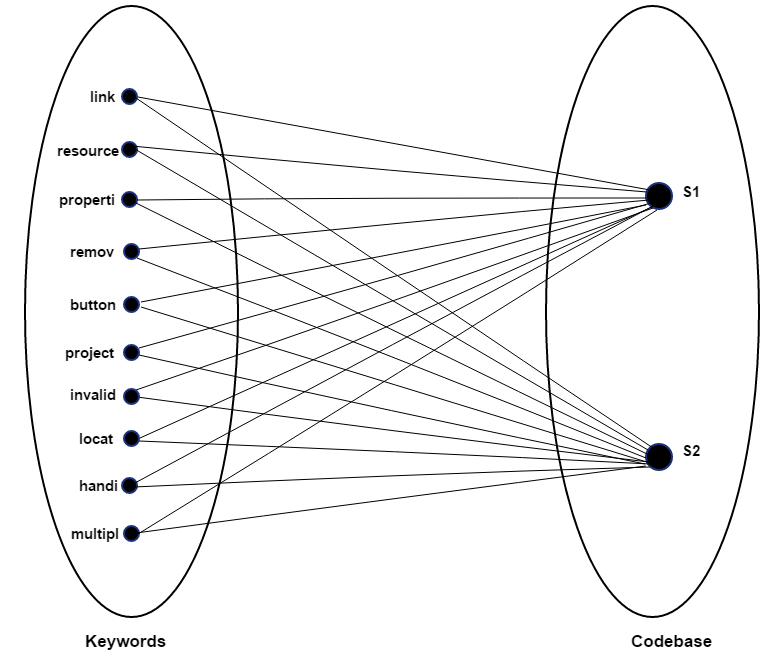
\includegraphics[scale=0.53]{BGraph2}
	\caption{A Bipartite Graph Constructed for Bug \#46669. 
		%Here, S1 represents %\textit{org.eclipse.ui.internal.ide.IDEWorkbenchMessages.java} and S2 represents %\textit{org.eclipse.ui.internal.ide.dialogs.LinkedResourceEditor.java}
	}
	\label{fig:BipartiteGraph}
\end{figure}


In our work, two groups correspond to keywords and codebase. Hence, nether two keywords nor two source files can be connected. There exist only one type of valid link, which can be established between a keyword and its corresponding sources. 
We construct a bipartite graph for a bug report (ID 322401) on the Eclipse UI Platform. Table \ref{tab:BugInfo2} shows the \textit{title} and \textit{description} of the bug report. The bipartite graph is presented in Figure \ref{fig:BipartiteGraph}. Note, that ten unique keywords are extracted from the bug report (i.e., from title and description) and are connected through edges with their corresponding change codes (i.e., $S1$ represents 
%org.eclipse.ui.internal.ide.
\textit{IDEWorkbenchMessages.java} and $S2$ represents 
%org.eclipse.ui.internal.ide.dialogs.
\textit{LinkedResourceEditor.java}). 
\subsection{Bug Localization Using VSM and Association Scores}

The system diagram for this part has illustrated in Figure \ref{fig:systemDiagram}(b), which 
%In BLuAMIR, we perform bug localization in two different ways - Approach I 
is based on the combination of VSM and association scores (i.e., Figure \ref{fig:systemDiagram}(b)).
%(b)) and Approach II is based on rVSM, Simi and association scores (i.e., Figure \ref{fig:systemDiagram} (c)). 
We have constructed an association map databases from keywords collected from bug report into its corresponding source code information in Section \ref{sec:MapConstruction}.
For the candidate keyword tokens for the initial query, we exploit association map database (i.e., keyword-source code links) and retrieve the relevant source code files. We use some heuristic functions in order to combine two ranks and recommend buggy relevant source files. Algorithm \ref{algo:localization} shows pseudo-code for our bug localization approach.


\begin{algorithm}[!t]
	\caption{Bug Localization using Association Mapping Database and Information Retrieval}
	\label{algo:localization}
	\begin{algorithmic}[1]
		\Procedure{BugLocalization}{$Q$, $SCrepo$, $MAP_{KS}$}
		
		\Comment{$Q$: a bug report query}
		
		\Comment{$SCrepo$: a source code repository}
	
		\Comment{$Map_{KS}$: association map created from Algorithm \ref{algo:map}}
		
		%\Comment{creating adjacency map database from the bug reports collection}
		%\State $MAP_{adj} \gets$ createAdjacencyDatabase($BRC$)
		%\Comment{creating a map that links keywords into their bug ids}
		\State $RankedR \gets$ \{\}
		\Comment{List of recommended buggy files}
		
		\State $Index \gets$ createIndex($SCrepo$)
		
		\Comment{Create Index from source code corpus}
		
		\State $Score_{Assoc} \gets$ calculateAssociationScore($Q$,$MAP_{bk}$)
		
		\Comment{Calculate Association score}
		
		\State $Score_{VSM} \gets$ calculateVSMscore($Q$,$Index$)
		
		\Comment{Calculate VSM score}
		
		%\Comment{Linking keywords into change source code}
		%\LineComment{preprocess the collected keywords}
		%\For{Keyword $K_i \in$ $K$}
		\State $SC_{Assoc} \gets$ collectSCodeWithAssocScore($Score_{Assoc}$)
		
		\Comment{Collect Source Codes for which association score is computed}
		
		\For{SourceCode $SC_{_i}$ $\in$ $SC_{Assoc}$}
		\State $Rank_{Assoc_{i}} \gets$ retrieveAssocScore ($Score_{Assoc}$)
		
		\Comment{retrieve association score for each source file}
		
		\State $Rank_{VSM_{i}} \gets$ retrieveVSMScore ($Score_{VSM}$)
		
		\Comment{retrieve VSM score for the same source file}
		
		\State $CombineS[SC_{i}]\gets Rank_{Assoc_{i}} + Rank_{VSM_{i}}$
		
		\Comment{Combine both scores utilizing a heuristic metric}
	
		\EndFor
	
		
		
		\State $RankedR \gets$ retrieveTopRSF ($CombineS[SC_{i}]$)
		
		\Comment{Sort combine score and retrieve top ranked buggy files}
		%\LineComment{put them into map}
		%\State $MAP \gets$ mapping()
		\State \textbf{return} $RankedR$
		\EndProcedure
	\end{algorithmic}
\end{algorithm}

%However, for simplicity we represent the former approach (i.e., Approach I) in our proposed schematic diagram in Fig. \ref{fig:systemDiagram}(b).
%In this approach, we calculate VSM and Co-occurence ranks in order to recommend buggy source codes for a given newly reported bug. 
%On the other hand,
%in our second approach, we work with three different ranks i.e., rVSM, Simi and Co-occurence. We replicate an existing technique proposed by \citet{Jian} for computing rVSM and Similarity scores. Basically, both VSM and rVSM are TF-IDF based score, which is measured between query and source code files.
%On the other hand, Simi score refers to that fact that if a bug is similar to another bug, then they both tend to relate to same sources. However, we describe both scores in Section \ref{Sec:Localize}.


%\section{Existing Approaches}\label{sec:existing}
%As in our proposed tool, we combine lexical similarity with word co-occurence score, here we discuss TF-IDF based bug localization approach.
%\subsection{Lexical Similarity Based Bug Localization Technique:}
%In this technique, each source code file is ranked based on source code file scores. Source code file contains words those can be also occurred in the bug reports. This is considered as a hint to locate buggy files. 
%%If a new bug is similar to a given previously located bug, then there is a possibility that the source code files located for the past bug can provide useful information in finding buggy files for that new bug.
%For locating a new bug we compute similarity scores for all source code files for a given project. However, we need to focus on some concepts which are required to understand our proposed system. They are described as follows:

%\textbf{Ranking based on Classical Vector Space Mode:}
%The basic idea of a VSM (Vector Space Model) or TF-IDF model is that the weight of a term in a document is increasing with its occurrence frequency in this specific document and decreasing with its occurrence frequency in other documents \cite{Jian}.
%In our proposed approach we have used both classical Vector Space Model (VSM) and revised Vector Space Model (rVSM) proposed by \citet{Jian} in order to index and rank source code files. 
%In classic VSM, \textit{tf} and \textit{idf} are defined as follows:
%\begin{equation}
%tf(t,d)=\frac{f_{td}}{\#terms}, idf(t)=log\frac{\#doc}{n_{t}}
%\end{equation}
%Here \textit{tf} is the term frequency of each unique term \textit{t} in a document \textit{d} and \textit{f\textsubscript{td}} is the number of times term \textit{t} appears in document \textit{d}.
%So the equation of classical VSM model is as follows
%\begin{multline}\label{VSMequation}
%VSMScore(q,d)= cos(q,d) =
%\\
%\frac{1}{\sqrt{\sum_{t\epsilon q}}((\frac{f_{tq}}{\#terms})\times log(\frac{\#docs}{n_{t}}))^{^{2}}}\times 
%\\
%\frac{1}{\sqrt{\sum_{t\epsilon d}((\frac{f_{td}}{\#terms})\times log(\frac{\#docs}{n_{t}}))^{2}}}\times
%\\
%\sum_{t\epsilon q\bigcap d}(\frac{f_{tq}}{\#terms})\times (\frac{f_{td}}{\#terms})\times log(\frac{\#docs}{n_{t}})^{2}
%\end{multline}
%This \textit{VSM} score is calculated for each query bug report \textit{q} against every document \textit{d} in the corpus. However, in the above equation \textit{\#terms} refers to the total number of terms in a corpus, \textit{n\textsubscript{t}} is the number of documents where term \textit{t} occurs.

%\textbf{Ranking based on Revised Vector Space Mode:}
%The main difference between classic VSM and revised VSM is that in case of revised version logarithm variant is used in computing term frequency. The equation for calculating term frequency is:
%\begin{equation}
%tf(t,d)=log(f_{td})+1
%\end{equation}
%So the new equation of revised VSM model is as follows:
%\begin{multline}\label{rVSMequation}
%rVSMScore(q,d)=g(\#term)\times cos(q,d)
%\\
%\frac{1}{1+e^{-N(\#terms))}}\times \frac{1}{\sqrt{\sum_{t\epsilon q}}((logf_{tq}+1)\times log(\frac{\#docs}{n_{t}}))^{^{2}}}\times 
%\\
%\frac{1}{\sqrt{\sum_{t\epsilon d}((log {f_{td}+1})\times log(\frac{\#docs}{n_{t}}))^{2}}}\times
%\\
%\sum_{t\epsilon q\bigcap d}(logf_{tq}+1)\times (logf_{td}+1)\times log(\frac{\#docs}{n_{t}})^{2}
%\end{multline}
%%\end{equation}
%This \textit{rVSM} score is calculated for each query bug report \textit{q} against every document \textit{d} in the corpus. However, in the above equation \textit{\#terms} refers to the total number of terms in a corpus, \textit{n\textsubscript{t}} is the number of documents where term \textit{t} occurs.
%
%\textbf{Ranking based on similar bug information}
%\begin{figure}
%	\centering
%	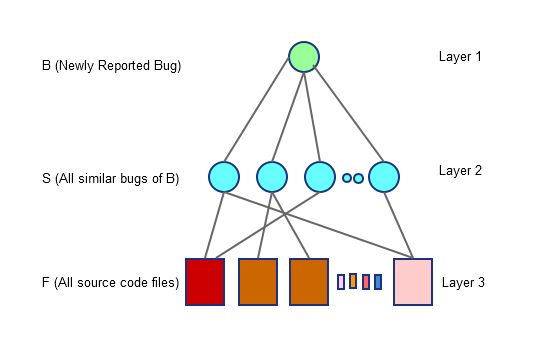
\includegraphics[scale=0.65]{3layers}
%	\caption{Bug and its Similar Bug Relationship with Source Code Files:}
%	\label{fig:BSBR}
%\end{figure}
%The assumption of this ranking is similar bugs of a given bug tend to modify similar source code files. Here, we construct a 3-layer architecture as described in \cite{Jian}. In the top layer (layer 1) there is a bug \textit{B} which represents a newly reported bug. All previously fixed bug reports which have non-negative similarity with bug  \textit{B} are presented in second layer. In third layer all source code files are shown. In order to resolve each bug in second layer some files in the corpus were modified or changed, which are indicated by a link between layer 2 and layer 3. Foe all source code files in layer 3, similarity score is computed, which can be referred to as degree of similarity. The score can be defined as:
%
%\begin{equation}\label{Simiequation}
%SimiScore=\sum_{All S_{i} that connect to F_{j}}(Similarity(B,S_{i})/n_{i})
%\end{equation} 
%Here, similarity between newly reported bug \textit{B} and previously fixed bug \textit{S\textsubscript{i}} is calculated based on cosine similarity measure and \textit{n\textsubscript{i}} is the total number of link \textit{S\textsubscript{i}} has with source code files in layer 3.

%%\subsection
%\textbf{Combining Both Ranks:}
%We combine the both scores based on source code score and similar bugs score as in \cite{Jian} as follows:
%\begin{equation}
%FinalScore=(1-\alpha )\times N(rVSMScore)+\alpha \times N(SimiScore)
%\end{equation}



%\subsection{LDA Topic Based Bug Localization Technique:}
%The main assumption behind this technique is the textual content of the bug reports and their associated buggy source code files tend to describe some common technical aspects. So, if  we could identify the technical topics extracted from both bug reports and source codes, we could recommend the files shared technical topics with the newly reported bug reports. If a newly reported bug has similar technical topics with some previously fixed bug reports, the fixed files could be a good candidate files for newly reported bug.
%
%LDA (Latent Dirichlet Allocation) is a probabilistic and fully generative topic model. It is used to extract latent (i.e., hidden) topics, which are presented in a collection of documents. It also model each document as a finite mixture over the set of topics [add link here]. In LDA, similarity between a document \textit{d} and a query \textit{q} is computed as the conditional probability of the query given that document \cite{Lukins2}.
%
%\begin{equation}
%Sim(q,d_{i})=P(q|d_{i})=\prod_{q_{k}\epsilon q}P(q_{k}|d_{i})
%\end{equation}
%
%Here \textit{q\textsubscript{k}} is the \textit{k}th word in the query {q} Thus, a document (i.e., source code file) is relevant to a query if it has a high probability of generating the words in the query.
%
%We perform the following steps in order to localize buggy files for newly reported bug using LDA based approach:
%
%\begin{itemize}
%	\item Apply topic modeling on the source code files. The output contains a certain number of topics and some associated keywords for each topic. We also get some other distribution files such as document-topic, word-topic etc.
%	\item Now work with the documents topic distribution file. Make a list of source code documents or files for each topic. So, we wiill have a list that contain all topics and their associated source code documents.
%	\item Here our query is the newly reported bug. This contains information in the bug reports such as title and short description etc. We all do inference for this query using a topic modeling tool. It will extract all topic associated with the query (i.e., newly reported bug).
%	\item Now we need to work with topic keywords. We are going to perform a comparison between newly reported bug or the given query and source code files using topic information. That means we will compare topic-keywords associated with topics inferred for the query with topic-keywords of each topic extracted from source code documents.
%	\item We will rank them based on topic-keyword similarity. So, now we know which are the top most topics, and we already have information regarding topic-document relationship, we will retrieve all source code files associated with all those top most topic as recommended buggy files.
%	%\item A detailed description of methodologies for visualizing topic evolution extracted from bug reports.
%	%\item A detailed description of methodologies for visualizing bug report extractive summaries.
%	%\item Evaluation of visualized bug report extractive summary by conducting a task-oriented user study.
%\end{itemize}


%\section{Part I: Association Map Database Construction}\label{sec:MapConstruction}
%%Our proposed approach consists of two parts - (i) constructing association map databases and (ii) retrieve relevant buggy source code files. 
%
%%\subsection{Part I: Construction of Association Map Database Between Bug Reports and Source Files}
%In this part, we construct an association map databases - between keywords and corresponding source code links extracted from bug reports and commit messages respectively. This section can be further divided into several parts: keyword extraction from bug reports, source code information extraction from commit logs, keyword- source code linking. We also create an algorithm for creating association map database between bug report keywords into their buggy source files, which is given in Algorithm \ref{algo:map}. However, several steps of map database construction are discussed in the followings:





%\section{Part II: Localizing Buggy Source Code Files} \label{Sec:Localize}
%In this part, we combine existing two lexical similarity based bug localization approaches with our proposed keyword-source co-occurence relation. One is with VSM score and other one is with rVSM and Simi ranks which are proposed in BugLocator \cite{Jian}. So, there are two sub parts of this section.
%\subsection{Approach I: Combinition of VSM and Co-occurence Rank:}
For locating a new bug we compute similarity scores for all source code files for a given project. However, we need to focus on some concepts which are required to understand our proposed system. They are described as follows:

\textbf{Association Scores Calculation}
A query typically contains several keywords or words. For each keyword, we look for relevant source files in the keyword-source files association map. We assume these files are relevant because we created the map between the content of bug reports and their buggy source files for previously fixed bug reports. When we analysis these links for all keywords in a query, a relevant file can be found from the association relationship more than once. Therefore, we then normalize the frequency of source files using standard TFIDF normalization technique. Finally we recommend first Top-K files with their association. The equation for computing association score is given belows:
\begin{equation}\label{CoOccequation}
AssociationScore=\sum_{All S_{i} that connect to W_{j}}(Link(W{j},S_{i}))
\end{equation}
Here, the link $Link(W{j},S_{i})$ between keyword and source file is 1 if they are connected in the association map and 0 otherwise. This step is done in line 4 of Algorithm \ref{algo:localization}.

\textbf{Vector Space Model:}
The vector space model (VSM) is a classical method for constructing vector representations for documents \cite{Salton}. 
It encodes a document collection by a term-by-document matrix. It represents one type of text unit (documents) by its association with the other type of text unit (terms). Here, the association is calculated by explicit evidence based on term occurrences in the documents.
The similarity between documents is computed by the cosine or inner product between corresponding vectors.

\textbf{VSM Score Calculation:}
Source code file contains words those can be also occurred in the bug reports. This is considered as a hint to locate buggy files. 
%If a new bug is similar to a given previously located bug, then there is a possibility that the source code files located for the past bug can provide useful information in finding buggy files for that new bug.
The basic idea of a VSM (Vector Space Model) is that the similarity between documents is computed by the cosine or inner product between terms collected from a query and a source document.
The weight of a term in a document increases with its occurrence frequency in this specific document and decreases with its occurrence frequency in other documents.
%In our proposed approach we have used both classical Vector Space Model (VSM)  and revised Vector Space Model (rVSM) proposed by \citet{Jian} in order to index and rank source code files. 
In classic VSM, {$tf$} (i.e., term frequency) and {$idf$} (i.e., inverse document frequency) are defined as follows:
\begin{equation}
tf(t,d)=\frac{f_{td}}{\#terms}, idf(t)=log\frac{\#doc}{n_{t}}
\end{equation}
Here $tf$ is the term frequency of each unique term {$t$} in a document {$d$} and {$f\textsubscript{td}$} is the number of times term {$t$} appears in document {$d$}.
So the equation of classical VSM model is as follows
\begin{multline}\label{VSMequation}
VSMScore(q,d)= cos(q,d) =
\\
\frac{1}{\sqrt{\sum_{t\epsilon q}}((\frac{f_{tq}}{\#terms})\times log(\frac{\#docs}{n_{t}}))^{^{2}}}\times 
\\
\frac{1}{\sqrt{\sum_{t\epsilon d}((\frac{f_{td}}{\#terms})\times log(\frac{\#docs}{n_{t}}))^{2}}}\times
\\
\sum_{t\epsilon q\bigcap d}(\frac{f_{tq}}{\#terms})\times (\frac{f_{td}}{\#terms})\times log(\frac{\#docs}{n_{t}})^{2}
\end{multline}
This \textit{VSM} score is calculated for each query bug report {$q$} against every document {$d$} in the corpus. However, in the above equation {$\#terms$} refers to the total number of terms in a corpus, {$n\textsubscript{t}$} is the number of documents where term {$t$} occurs. This score is calculated in line 5 of Algorithm \ref{algo:localization},




\textbf{Final Score Calculation}
We compute VSM score using Appache Lucene library. Then we combine that score with our association using equation \ref{equationVSMme}.
\begin{multline}\label{equationVSMme}
FinalScore=(1-\alpha )\times N(VSMScore)+ \\
\alpha \times N(AssociationScore)
\end{multline}
Here, the weighting factor $\alpha$ varies from 0.2 to 0.4, for which we discuss results in the experiment section \ref{RQ2Answer}. 

We combine both scores using equation \ref{equationVSMme} in Algorithm \ref{algo:localization} line 7-11. Finally, top ranked recommended buggy files are retrieved, which is done line 12 of Algorithm \ref{algo:localization}.





\section{Experiment and Discussion} \label{sec:expANDdiss}
In this section, at first we discuss detail of our data set, then we describe the evaluation metrics, research questions and finally we present our experimental results.




%\begin{table}[htbp]
%\caption{Table Type Styles}
%\begin{center}
%\begin{tabular}{|c|c|c|c|}
%\hline
%\textbf{Table}&\multicolumn{3}{|c|}{\textbf{Table Column Head}} \\
%\cline{2-4} 
%\textbf{Head} & \textbf{\textit{Table column subhead}}& \textbf{\textit{Subhead}}& \textbf{\textit{Subhead}} \\
%\hline
%copy& More table copy$^{\mathrm{a}}$& &  \\
%\hline
%\multicolumn{4}{l}{$^{\mathrm{a}}$Sample of a Table footnote.}
%\end{tabular}
%\label{tab1}
%\end{center}
%\end{table}



\subsection{Experimental Dataset}
We work with four different dataset - Eclipse, AspectJ, SWT aand Zxing.
In order to evaluate our proposed tool we have used the same four dataset that \citet{Jian} and \citet{Saha} used
to evaluate BugLocator and BLUiR respectively. This dataset contains 3479 bug reports in total from four popular open source projects–Eclipse, SWT, AspectJ and ZXing along with the information of fixed files for those bugs.
The detail of our dataset is presented in \ref{tab:DDSl}. 
Eclipse\footnote{https://bugs.eclipse.org/} is a well-known large-scale open source system and it is widely used in empirical software engineering research.
SWT\footnote{http://www.eclipse.org/swt/} is a component of Eclipse.
The AspectJ\footnote{http://www.st.cs.uni-saarland.de/ibugs/} project is a part of the iBUGs public dataset provided by the University of Saarland. 
Zxing\footnote{http://code.google.com/p/zxing/} is an android based project maintained by google.
%We work with Eclipse data set which is a popular IDE for Java. 
%We downloaed a git based Eclipse project from git repository \footnote{https://git.eclipse.org/c/platform/eclipse.platform.ui.git/}. We work with Eclipse Platform UI project. 
%These source codes are contained in our source code repository. 
%On the other hand, currently Eclipse Platform UI project contains more than 10K number of bugs where we only work with the bugs which are fixed. 
We create quires from each bugs considering their title and short summary (i.e., description).
%We have two parts in our corpus. One is source code files downloaded as git based project and another part is bug reports collection. All bug reports are collected from. 
In order to obtain the links between previously fixed bugs and source code files, we analyze git project commit message. We ran through all commit messages and track Bug IDs associated with examined source code files. Then we construct the association map between keywords extracted from bug reports and their source code links. During creating the map we have noticed some bug reports do not contain their fixed source files in codebase. So, we discarded those bug reports which yield total 3431 bug reports as depicted in table \ref{tab:DDSl}.
 

\begin{table}[htbp]
	\caption{Description of Data Sets}
	\label{tab:DDSl}
	%\centering
	\begin{center}
		\begin{tabular}{ p{1cm} | p{2.5cm} | p{1.5cm} | p{.75cm} | p{.75cm} }
			\hline
			\textbf{Project Name}  & \textbf{Description} & \textbf{Study Period}& \textbf{\#Fixed Bugs} & \textbf{\#Source Files}\\
			\hline
			%{Eclipse Platform Ant} & Popular IDE for Java & Nov 2001 - April 2010 & {3855} & 11732\\ \hline
		 \hline
				
			{Eclipse (v3.1)} & An open development platform for Java & Oct 2004 - Mar 2011 & {3071} & 11831\\ \hline
			SWT (V 3.1)& An open source widget toolkit for Java & Oct 2004 - Apr 2010 & 98 &  484\\ \hline
			AspectJ& Aspect-oriented extension to Java & July 2002 - Oct 2006 & 244 & 3519 \\ \hline
			ZXing & A barcode image processing library for Android Application & Mar 2010 - Sep 2010 & 20 & 391 \\
			\hline
			
		\end{tabular}
	\end{center}
	%\centering
\end{table}
\subsection{Evaluation Metrices}
To measure the effectiveness of the proposed bug localization approach, we use the following metrics:

\textbf{Ton N-Rank (Hit@N):} It represents the number of bug, for which their associated files are returned in a ranked list. Here, \textit{N} may be 1, 5 or 10. We assume that if at least one associated file is presented in the resulted ranked list, then the given bug is located. The higher the metric value, the better the bug localization performance.

\textbf{MRR (Mean Reciprocal Rank)}
The reciprocal rank of a query is the multiplicative inverse of the rank of the first correct answer. So mean reciprocal rank is the average of the reciprocal ranks of results of a set of queries $Q$
\begin{equation}
MRR=\frac{1}{\left | Q \right |}\sum_{i=1}^{\left | Q \right |}\frac{1}{rank_{i}}
\end{equation}
where $rank_i$ is the position of the first buggy file in the returned ranked files for the first query in $Q$.

\textbf{MAP (Mean Average Precision)}
Mean Average Precision is the most commonly used IR metric to evaluate ranking approaches. It considers the ranks of all buggy files into consideration. So, MAP emphasizes all of the buggy files instead of only the first one.
MAP for a set of queries is the mean of the average precision scores for each query. The average precision of a single query is computed as:
\begin{equation}
AP=\sum_{k=1}^{M}\frac{P(k)\times pos(k)}{number \, of \, positive \, instances}
\end{equation}
where $k$ is a rank in the returned ranked files, $M$ is the number of ranked files and $pos(k)$ indicates whether the $k_{th}$ file is a buggy file or not. $P(k)$ is the precision at a given top $k$ files and is computed as follows:
\begin{equation}
P(k)=\frac{\#buggy \, Files}{k}
\end{equation}

%\textbf{Wilcoxon signed-rank test}
%The Wilcoxon signed-rank test is a non-parametric statistical hypothesis test used to compare two related samples, matched samples, or repeated measurements on a single sample to assess whether their population mean ranks differ. We perform this test with the help of \footnote{https://www.socscistatistics.com/tests/signedranks/Default.aspx}.
%
%\textbf{Cross Validation}
%We divide our query data into k number of sets. Typically k is 10, but we work with k =5 and k=10. Each set contains a training set and tesing set. Training data is used to create mapping between keywords extracted from bug reports and source code files. 10-fold-cross validation data is presented in table \ref{tab:Performance1} and table \ref{tab:Performance2}.


\subsection{Research Questions}
Our proposed tool-BLuAMIR are designed to  answer the following research questions.
\begin{itemize}
	%\item RQ1: How many bugs can be successfully located by BLuAMIR?
	\item RQ1: (a) How does our proposed approach-BLuAMIR perform in Bug Localization? (b) How does our proposed association score affect its performance?
	\item RQ2: Does our proposed approach-BLuAMIR resolve the vocabulary missmatch problem and how?
	\item RQ3: Does our proposed approach-BLuAMIR eliminate large files problem and how?
	\item RQ4: Is BLuAMIR comparable with the state-of-the-art techniques in identifying buggy files?
\end{itemize}






\subsection{Experimental Results}
During experiment, we evaluate our proposed approach in different ways. To create mapping between bug report keywords and source files, we consider three different options - (1) including only title or summary of a bug report in creating corpus, (2) in addition with title we also include description field of a bug report and (3) full content of a bug report could be an option. Neither option 1 nor 3 provides better result and option 2 optimized the performance. We explain this in a way that providing only title of a big report conveys very little information. On the other hand, including full content of a bug report also create too much information that contains huge noise data and also takes longer time during mapping them into source code files. Therefore, title and description of a bug report optimized those two options. However, considering title and description did not get rid of noise and therefore we discard all keywords that happen to exist in 25\% or more documents in the corpus.

%However, we divide our experimental result into two parts based on experimented dataset. 
%We implemented BLuAMIR by two different approaches. 
First, we compare the performance of BLuAMIR with replicated basic VSM based bug localization technique for Eclipse dataset. We also compare the performance between replicated LSI \citet{MarcusLSI} and BLuAMIR for AspectJ, SWT and ZXing datasets. The detail of this comparison is presented in the following subsection.
%For that, we replicate BugLocator proposed by \citet{Jian}.
Second, we compare the performance of BLuAMIR with three state of the arts techniques, BugScout \cite{Nguyen}, BugLocator \cite{Jian} and BLUiR \cite{Saha} for the same dataset as in \cite{Jian}. Here we collect the results reported by the authors and then compare the performance with BLuAMIR. We also answer our research questions in the following subsections.

%\subsection{Comparison Between Replicated BugLocator and BLuAMIR}
%%\subsection{Bug Localization using rVSM, Simi and Association Scores:}
%First, we replicate an existing technique (i.e., BugLocator) proposed by \citet{Jian}. 
%\citet{Jian} uses
%revised Vector Space Model (rVSM) and Simi scores in order to index and rank source code files.
%Second, we combine our proposed association score with these two scores ranks (i.e., rVSM, Simi). Finally, we perform comparison between replicated BugLocator with this combined scores in terms of Top-1, Top-5, Top-10, MRR and MAP. Ranking based on rVSM and Simi and our combined approach are depicted as follows.
%%If a new bug is similar to a given previously located bug, then there is a possibility that the source code files located for the past bug can provide useful information in finding buggy files for that new bug.
%%On the other hand, Simi score refers to that fact that if a bug is similar to another bug, then they both tend to relate to same sources. However, we describe both scores in Section \ref{Sec:Localize}
%
%\textbf{Ranking based on Revised Vector Space Model:}
%The main difference between classic VSM and revised VSM is that in case of revised version logarithm variant is used in computing term frequency. The equation \cite{Jian} for calculating term frequency is:
%\begin{equation}
%tf(t,d)=log(f_{td})+1
%\end{equation}
%So the new equation of revised VSM model is as follows:
%\begin{multline}\label{rVSMequation}
%rVSMScore(q,d)=g(\#term)\times cos(q,d)
%\\
%\frac{1}{1+e^{-N(\#terms))}}\times \frac{1}{\sqrt{\sum_{t\epsilon q}}((logf_{tq}+1)\times log(\frac{\#docs}{n_{t}}))^{^{2}}}\times 
%\\
%\frac{1}{\sqrt{\sum_{t\epsilon d}((log {f_{td}+1})\times log(\frac{\#docs}{n_{t}}))^{2}}}\times
%\\
%\sum_{t\epsilon q\bigcap d}(logf_{tq}+1)\times (logf_{td}+1)\times log(\frac{\#docs}{n_{t}})^{2}
%\end{multline}
%%\end{equation}
%This \textit{rVSM} score is calculated for each query bug report {$q$} against every document {$d$} in the corpus. However, in the above equation {$\#terms$} refers to the total number of terms in a corpus, {$n\textsubscript{t}$} is the number of documents where term {$t$} occurs.
\begin{figure*}
	\begin{subfigure}
		\centering
		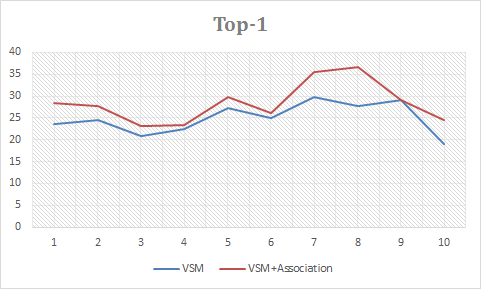
\includegraphics[width=.33\textwidth]{VSM+AssoTop-1}
		%\caption {Performance Comparison between VSM and VSM+Association for Top-1 Retrieval}
		%\label{fig:VSM+AssoTop-1}...
	\end{subfigure}
	\begin{subfigure} 
		\centering
		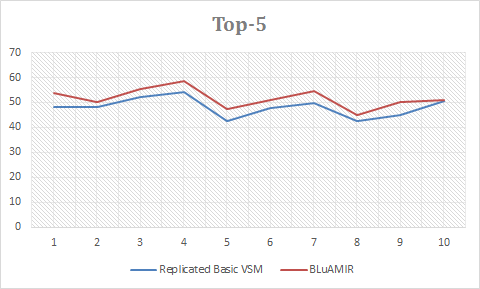
\includegraphics[width=.33\textwidth]{VSM+AssoTop-5}
		%\caption {Performance Comparison between VSM and VSM+Association for Top-5 Retrieval}
		%\label{fig:VSM+AssoTop-5}
	\end{subfigure}
	\begin{subfigure} 
		\centering
		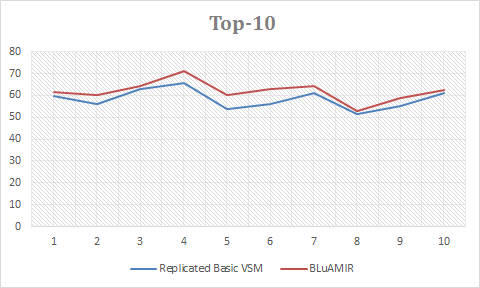
\includegraphics[width=.33\textwidth]{VSM+AssoTop-10}
		%\caption {Performance Comparison between VSM and VSM+Association for Top-10 Retrieval}
		%\label{fig:VSM+AssoTop-10}
	\end{subfigure}
	
	\caption {Performance Comparison between replicated basic VSM and BLuAMIR for Top-1, Top-5 and Top-10 Retrieval}
	\label{fig:VSM+AssoTopK}
\end{figure*}
\begin{figure}
	\centering
	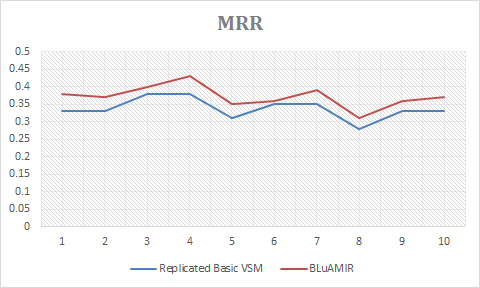
\includegraphics[scale=0.70]{VSM+AssoTop-MRR}
	\caption {MRR Comparison between replicated basic VSM and BLuAMIR}
	\label{fig:VSM+AssoTop-MRR}
\end{figure}
\begin{figure}
	\centering
	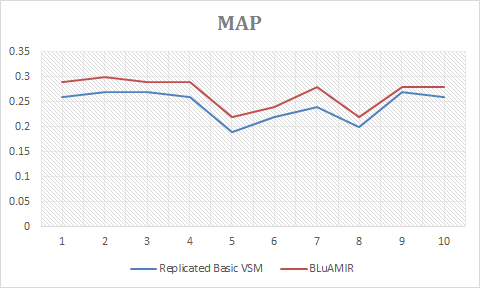
\includegraphics[scale=0.70]{VSM+AssoTop-MAP}
	\caption {MAP Comparison between replicated basic VSM and BLuAMIR}
	\label{fig:VSM+AssoTop-MAP}
\end{figure}
%
%\textbf{Ranking based on similar bug information}
%\begin{figure}
%	\centering
%	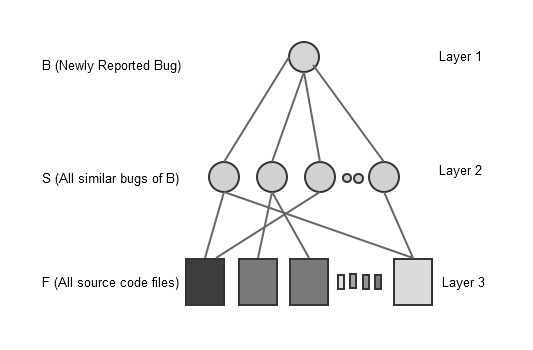
\includegraphics[scale=0.48]{3layers-Gray}
%	\caption{Bug and its Similar Bug Relationship with Source Code Files:}
%	\label{fig:BSBR}
%\end{figure}
%The assumption is if a new bug is similar to a given previously located bug, then there is a possibility that the source code files located for the past bug can provide useful information in finding buggy files for that new bug.. Here, we construct a 3-layer architecture as described in \cite{Jian}. In the top layer (layer 1) there is a bug \textit{B} which represents a newly reported bug. All previously fixed bug reports which have non-negative similarity with bug  \textit{B} are presented in second layer. In third layer all source code files are shown. In order to resolve each bug in second layer some files in the corpus were modified or changed, which are indicated by a link between layer 2 and layer 3. Foe all source code files in layer 3, similarity score is computed, which can be referred to as degree of similarity. The score can be defined as:
%
%\begin{equation}\label{Simiequation}
%SimiScore=\sum_{All S_{i} that connect to F_{j}}(Similarity(B,S_{i})/n_{i})
%\end{equation} 
%Here, similarity between newly reported bug {$B$} and previously fixed bug {$S\textsubscript{i}$} is calculated based on cosine similarity measure and {$n\textsubscript{i}$} is the total number of link {$S\textsubscript{i}$} has with source code files in layer 3.
%
%
%
%\textbf{Final Score Calculation}
%For each query, we compute the rVSM score against all source codes in the database using equation \ref{rVSMequation} and we also calculate Simi score using equation \ref{Simiequation}. Then we calculate association scores for the query using equation \ref{CoOccequation}.
%We finally combine the three ranks and for that we use three weighting factor {$\alpha$}, $\beta$ and $\gamma$.
%The final equation is given in equation \ref{equationBLme}.
%\begin{multline}\label{equationBLme}
%CombinedScore=\gamma \times N(rVSMScore)+
%\\ \beta \times N(SimiScore) + \alpha \times N(AssociationScore)
%\end{multline}
%We work with different values of $\alpha$, which are presented in the experiment section \ref{RQ2Answer}. We use value of 0.2 for $\beta$, varying $\alpha$ from 0.1 to 0.5 and thus, $\gamma$ from 0.7 to 0.3. So that they end up into 1.
%\subsection{Answering RQ1} \label{RQ1answer}
%To answer RQ1, we compare the performance of our proposed bug localization approach with two existing techniques - 1) VSM which is based on vector space model and 2) replicated BugLocaotor \cite{Jian} which is based on rVSM and Simi scores. 
%
%
%
%\begin{figure*}
%	\begin{subfigure}[b]{0.33\textwidth}
%		\centering
%		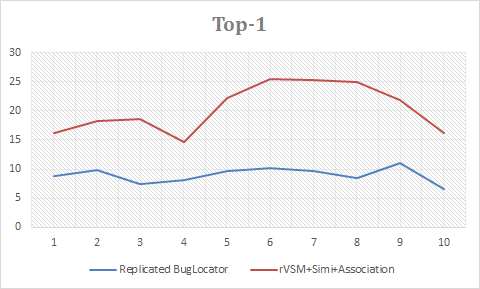
\includegraphics[width=\textwidth]{RBL+rSAssoTop-1}
%		%\caption {Performance Comparison between VSM and VSM+Association for Top-1 Retrieval}
%		%\label{fig:VSM+AssoTop-1}...
%	\end{subfigure}
%	\begin{subfigure} [b]{0.33\textwidth}
%		\centering
%		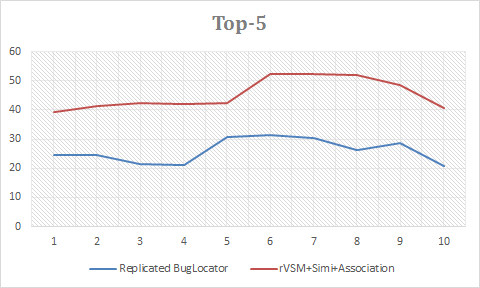
\includegraphics[width=\textwidth]{RBL+rSAssoTop-5}
%		%\caption {Performance Comparison between VSM and VSM+Association for Top-5 Retrieval}
%		%\label{fig:VSM+AssoTop-5}
%	\end{subfigure}
%	\begin{subfigure} [b]{0.33\textwidth}
%		\centering
%		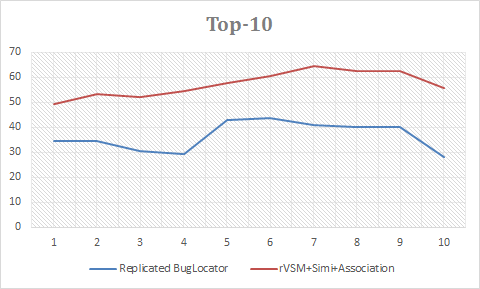
\includegraphics[width=\textwidth]{RBL+rSAssoTop-10}
%		%\caption {Performance Comparison between VSM and VSM+Association for Top-10 Retrieval}
%		%\label{fig:VSM+AssoTop-10}
%	\end{subfigure}
%	
%	\caption {Performance Comparison between Replicated BugLocator and rVSM+Simi+Association for Top-1, Top-5 and Top-10 Retrieval}
%	\label{fig:RepBL+AssoTopK}
%\end{figure*}
%\begin{figure}
%	\centering
%	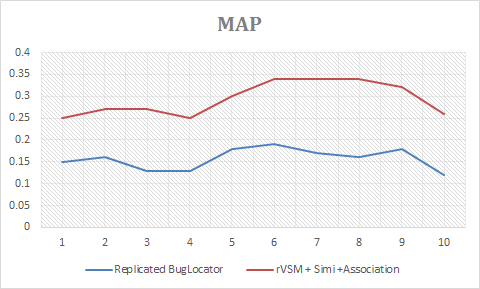
\includegraphics[scale=0.70]{RBL+rSAssoTop-MRR}
%	\caption {MRR Comparison between Replicated BugLocator and rVSM+Simi+Association}
%	\label{fig:RepBL+AssoTop-MRR}
%\end{figure}
%\begin{figure}
%	\centering
%	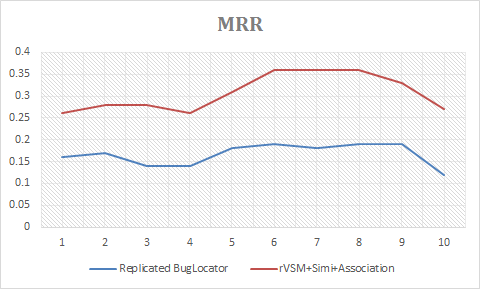
\includegraphics[scale=0.70]{RBL+rSAssoTop-MAP}
%	\caption {MAP Comparison between Replicated BugLocator and rVSM+Simi+Association}
%	\label{fig:RepBL+AssoTop-MAP}
%\end{figure}
\subsection{Answering RQ1} \label{RQ1answer}
To answer RQ1, we compare the performance of our proposed bug localization approach with two re-implemented existing techniques - 1) classic VSM which is based on vector space model and 2) replicated LSI \cite{MarcusLSI} which is based on latent semantic indexing.
\begin{table}[htbp]
	\centering
	\caption{Performance comparison of replicated basic VSM and proposed technique (BLuAMIR)}
	\label{tab:Performance2}
	\resizebox{3.5in}{!}{%
		\begin{tabular}{c|c|c|c|c|c|c}
			\hline
			%\begin{tabular}[c]{@{}c@{}}\#Bugs for \\ developing \\ map databases\end{tabular} &
			
			\begin{tabular}[c]{@{}c@{}} \textbf{\#Bugs} \\ \end{tabular} & 
			\begin{tabular}[c]{@{}c@{}}\#\textbf{Methodology} \\  \end{tabular} 
			& 
			\begin{tabular}[c]{@{}c@{}}\textbf{Top 1}\\ \%\end{tabular} & \begin{tabular}[c]{@{}c@{}}\textbf{Top 5}\\ \%\end{tabular} & \begin{tabular}[c]{@{}c@{}}\textbf{Top 10}\\ \%\end{tabular} & 
			\textbf{MRR@10} 
			& \textbf{MAP@10} \\ \hline \hline
			%			\multirow{2}{*}{1}& VSM & 23.67& 46.59&56.97& 0.33 & 0.32 \\ \cline{2-7}
			%			& VSM + Association & 28.40                                               & 51.77                                            & 60.06                                                &   0.38  & 0.36 \\ \hline
			%			\multirow{2}{*}{2}                                                                               & VSM & 24.62 & 48.05 & 57.96 & 0.34 & 0.34 \\  \cline{2-7}  &VSM + Association                                                                    & 27.63                                               & 53.15                                              & 61.26                                             &   0.38  &   0.37  \\ \hline
			%			\multirow{2}{*}{3}                                                                               & VSM & 20.78 & 40.96 & 51.20 & 0.30 & 0.29 \\  \cline{2-7}   &VSM + Association                                                                      & 23.12                                            & 46.85                                            & 59.76                                             &   0.34  &  0.32   \\ \hline
			%			\multirow{2}{*}{4}                                                                               & VSM & 22.52 & 42.94 & 53.75 & 0.32 & 0.31 \\   \cline{2-7} &VSM + Association                                                                    & 23.42                       & 49.25                       & 61.56                                                &  0.35   &  0.33  \\  \hline
			%			\multirow{2}{*}{5}                                                                               & VSM & 27.33 & 52.25 & 63.36 & 0.38 & 0.35 \\   \cline{2-7} &VSM + Association                                                                   & 29.73                                                 & 53.15                                                 & 62.16                                                  &  0.39   & 0.36     \\  \hline
			%			\multirow{2}{*}{6}                                                                               & VSM & 25.00 & 50.60 & 60.84 & 0.36 & 0.34 \\  \cline{2-7}  &VSM + Association
			%			&26.13 &
			%			51.65 &
			%			62.76 & 0.37 &
			%			0.35     \\  \hline 
			%			\multirow{2}{*}{7}                                                                               & VSM & 29.82 & 54.52 & 66.27 & 0.40 & 0.38 \\  \cline{2-7}  &VSM + Association
			%			
			%			&35.43 &
			%			60.96 &
			%			72.07 & 0.46 &
			%			0.44     \\  \hline
			%			\multirow{2}{*}{8}                                                                               & VSM & 27.79 & 51.36 & 60.73 & 0.38 & 0.36 \\  \cline{2-7}  &VSM + Association
			%			&36.64 &
			%			58.86 &
			%			67.87 & 0.46 &
			%			0.43    \\  \hline
			%			\multirow{2}{*}{9}                                                                               & VSM & 29.13 & 52.55 & 64.86 & 0.39 & 0.36 \\  \cline{2-7}   &VSM + Association
			%			&29.13 &
			%			61.86 &
			%			69.97 & 0.42 &
			%			0.40    \\  \hline
			%			\multirow{2}{*}{10}                                                                               & VSM & 19.03 & 39.58 & 51.34 & 0.28 & 0.26 \\  \cline{2-7}  &VSM + Association
			%			&24.62 &
			%			51.05 &
			%			63.06 & 0.36 &
			%			0.34    \\ \hline \hline
			\multirow{2}{*}{3071}                                                                               & Basic VSM & 23.09\% & 47.54\% & 57.57\% & 0.33 & 0.24 \\  \cline{2-7}   &VSM + Association     & 27.45\%                                                 & 53.79\%                                                 & 63.30\%                                                  &   0.38  &  0.27    \\ 
			\hline
	\end{tabular}}
	\centering
\end{table}
 

\textbf{VSM vs BLuAMIR}
In our proposed approach, we combine VSM score and association scores in order to produce a ranked result. We compare the performance of baseline VSM technique and our proposed combined approach on Eclipse dataset (i.e., 3071 bug reports). This performance comparison can assist us to investigate whether adding association score with VSM score can improve the bug localization performance or not. The comparison is presented in table \ref{tab:Performance2}. We also use a 10-fold cross validation i.e., divide all 3071 bug reports into-10 fold and perform train on total 9 folds and test on the rest fold. For 10-fold validated Eclipse codebase, we compute Hit@1, Hit@5, Hit@10 performance (presented in Fig \ref{fig:VSM+AssoTopK}) and MRR and MAP (shown in Fig \ref{fig:VSM+AssoTop-MRR} and Fig \ref{fig:VSM+AssoTop-MAP} respectively) for both approaches. In all cases our proposed approach outperforms VSM-based bug localization approach. The Hit@10 performance of our tool is 63.30\% whereas it is 58.26\% for VSM.
So. to answer our \textit{RQ1(a)}, we can go to Table \ref{tab:Performance2}, 63.30\% bugs are successfully located in Hit@10 for Eclipse dataset by BLuAMIR. This result also suggest that association score improves the retrieval performance of BLuAMIR (\textit{RQ1(b)}). 


We also compute Wilcoxon signed-rank test both for MRR and MAP. For MRR the {Z}-value is -2.8031. The {p}-value is 0.00512. The result is significant at p<=0.05. The W-value is 0. The critical value of W for N = 10 at p<=0.05 is 5. Therefore, the result is significant at p<=0.05.
For MAP - the {Z}-value is -2.8031. The {p}-value is 0.00512. The result is significant at p<=0.05. The W-value is 0. The critical value of W for N = 10 at p<=0.05 is 5. Therefore, the result is significant at p<=0.05.


\textbf{Replicated LSI vs BLuAMIR:}
Latent Semantic Indexing(LSI) is a VSM based method for indexing and representing aspects of the meanings of words, which reflects their usages. One of the problem with basic VSM that the user usually wants to retrieve on the basis of conceptual content. Most of the time individual words provide unreliable evidence about the conceptual topic or meaning of a document \cite{LSIindexing}. Therefore, to solve this problem \cite{Maletic, MarcusMaletic} utilize an advanced information retrieval technique (i.e., LSI) to extract the meaning of the documentation and source code. Based on any chosen similarity measure, they use this information to identify traceability links. However, we follow A LSI-based documentation to source code traceability links recovering technique proposed by \citet{MarcusLSI}.

At first we created a term-by-document matrix for corpus. Our corpus contains both the source code base and query bug reports. Then, we apply a Singular Value Decomposition (SVD) to construct a subspace (i.e., LSI subspace) \cite{SaltonMIR}. 
Then, we compute similarity between documents by the cosine or inner product between the corresponding vectors collected from LSI subspace matrix. Typically, two documents are considered similar if their corresponding vectors in the VSM spcae point in the same direction.
Note that we preprocess both source code and bug reports by spiliting each word, remove stop words etc. Then, we create the term-by-document matrix. However, finally we retrieve the rankled list of source codes for bug reports based on cosine similarity. We compare between replicated LSI and BLuAMIR for three datasets AspectJ, SWT and ZXing, which are depicted in Table \ref{tab:Performance1}.


\begin{table}[htbp]
	\caption{Performance of replicated LSI and BLuAMIR for AspectJ, SWT and ZXing dataset}
	\label{tab:Performance1}
	\centering
	\resizebox{3.4in}{!}{%
		\begin{tabular}{c|c|c|c|c|c|c}
			\hline
			%\begin{tabular}[c]{@{}c@{}}\#Bugs for \\ developing \\ map databases\end{tabular} &
			\begin{tabular}[c]{@{}c@{}}\#\textbf{System}  \\ \end{tabular} & \begin{tabular}[c]{@{}c@{}}\textbf{Methodology} \\ \end{tabular} &
			%\textbf{alpha} &
			%\textbf{beta}&
			%\textbf{gamma}& 
			\begin{tabular}[c]{@{}c@{}}\textbf{Top 1}\\ \%\end{tabular} & 
			\begin{tabular}[c]{@{}c@{}}\textbf{Top 5}\\ \%\end{tabular} & 
			\begin{tabular}[c]{@{}c@{}}\textbf{Top 10}\\ \%\end{tabular} &
			
			\begin{tabular}[c]{@{}c@{}} \textbf{MRR} \end{tabular} & 
			\begin{tabular}[c]{@{}c@{}} \textbf{MAP} \end{tabular} \\ \hline \hline
			%\multirow{2}{*}{1}  &Replicated BugLocator     &  8.88& 24.56&34.32& 0.16 & 0.15 \\  \cline{2-7}
			%& rVSM+Simi+ Association                                                                                                                                           & 16.27                                               & 39.35                                            & 49.41                                                &   0.26  & 0.25    \\ \hline
			%\multirow{2}{*}{2}  &Replicated BugLocator     &  9.9& 24.62&34.53& 0.17 & 0.16 \\ \cline{2-7}
			%& rVSM+Simi+ Association                                                                 & 18.32                                               & 41.44                                              & 53.45                                             &   0.28  &   0.27  \\ \hline
			%\multirow{2}{*}{3}  &Replicated BugLocator     &  7.50& 21.32&30.63& 0.14 & 0.13 \\ \cline{2-7}
			%& rVSM+Simi+ Association                                                                   & 18.62                                            & 42.34                                            & 52.25                                             &   0.28  &  0.27   \\  \hline
			%\multirow{2}{*}{4}  &Replicated BugLocator     &  8.1& 21.02&29.13& 0.14 & 0.13 \\  \cline{2-7}
			%& rVSM+Simi+ Association                                                                   & 14.71                       & 42.04                       & 54.35                                               &  0.26   &  0.25  \\  \hline
			%\multirow{2}{*}{5}  &Replicated BugLocator     &  9.6& 30.63&42.94& 0.18 & 0.18 \\  \cline{2-7}
			%& rVSM+Simi+ Association                                                                 & 22.22                                                 & 42.34                                                & 57.66                                                  &  0.31   & 0.30     \\ \hline
			%\multirow{2}{*}{6}  &Replicated BugLocator     &  10.21& 31.53&43.54& 0.19 & 0.19 \\  \cline{2-7}
			%& rVSM+Simi+ Association
			%&25.53 &
			%52.25 &
			%60.66 & 0.36 &
			%0.34     \\  \hline
			%\multirow{2}{*}{7}  &Replicated BugLocator     &  9.61& 30.33&40.84& 0.18 & 0.17 \\ \cline{2-7}
			%& rVSM+Simi+ Association
			%&25.22 &
			%52.25 &
			%64.56 & 0.36 &
			%0.34     \\  \hline
			%\multirow{2}{*}{8}  &Replicated BugLocator     &  8.4& 26.13&39.94& 0.19 & 0.16 \\ \cline{2-7}
			%& rVSM+Simi+ Association
			%&24.92 &
			%51.95 &
			%62.46 & 0.36 &
			%0.34    \\  \hline
			%\multirow{2}{*}{9}  &Replicated BugLocator     &  11.11& 28.83&40.24& 0.19 & 0.18 \\  \cline{2-7}
			%& rVSM+Simi+ Association
			%&21.92 &
			%48.65 &
			%62.46 & 0.33 &
			%0.32    \\  \hline
			%\multirow{2}{*}{10}  &Replicated BugLocator     &  6.6& 20.72&27.93& 0.12 & 0.12 \\  \cline{2-7}
			%& rVSM+Simi+ Association
			%&16.21 &
			%40.54 &
			%55.55 & 0.27 &
			%0.26    \\  \hline \hline
			\multirow{2}{*}{AspectJ}       &Replicated LSI     &  9.42\%& 24.59\%&29.10\%& 0.15 & 0.07  \\ \cline{2-7}
			& BLuAMIR                                                                                                                     & 33.20\%                                                 & 54.92\%                                                 & 66.39\%                                                  &   0.43  &  0.23    \\ 
			\hline
			\multirow{2}{*}{SWT}       &Replicated LSI     &  13.26\%& 30.61\%&53.06\%& 0.22 & 0.17  \\ \cline{2-7}
			& BLuAMIR                                                                                                                     & 45.93\%                                                 & 75.00\%                                                 & 82.29\%                                                  &   0.58  &  0.50    \\ 
			\hline
			\multirow{2}{*}{ZXing}       &Replicated LSI     &  15.00\%& 35.00\%&45.00\%& 0.23 & 0.21  \\ \cline{2-7}
			& BLuAMIR                                                                                                                     & 55.00\%                                                 & 80.00\%                                                 & 85.00\%                                                  &   0.67  &  0.62    \\ 
			\hline
	\end{tabular}}
	\centering
\end{table}


We compare the performance of our proposed approach in terms of Hit@k rank (depicted in Table \ref{tab:Performance2}) and MRR and MAP (shown in Box plot Fig \ref{box:LSI+AssoMRR} and Fig \ref{box:LSI+Asso-MAP} respectively). We can see that our proposed approach outperforms in all case. So, BLuAMIR successfully retrieve 66.39\%, 82.29\%, and 85.00\% bugs for AspectJ, SWT and ZXing datasets respectively in Hit@10. These results provide the answer of our \textit{RQ1(a)}. The box plots in Fig \ref{box:LSI+AssoMRR} and Fig \ref{box:LSI+Asso-MAP} also demonstrate that BLuAMIR performs better than the baseline in each of the measures with higher medians.
\begin{figure}
	\centering
	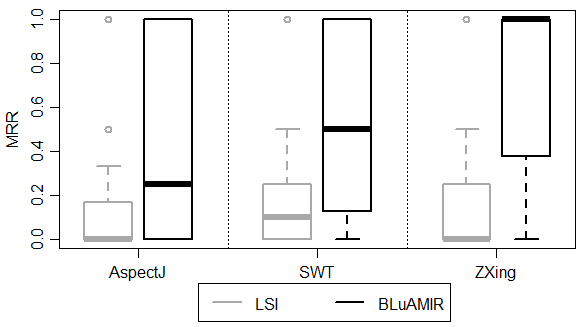
\includegraphics[scale=0.55]{comapre-mrr}
	\caption {MRR Comparison between replicated basic LSI and BLuAMIR for AspectJ, SWT and ZXing dataset}
	\label{box:LSI+AssoMRR}
\end{figure}
\begin{figure}
	\centering
	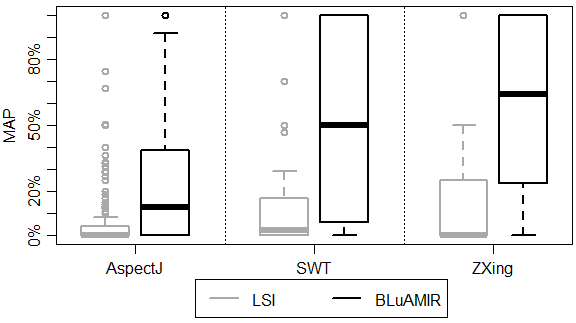
\includegraphics[scale=0.55]{compare-map-lsi-proposed}
	\caption {MAP Comparison between replicated basic LSI and BLuAMIR for AspectJ, SWT and ZXing dataset}
	\label{box:LSI+Asso-MAP}
\end{figure}
   


%We also compute Wilcoxon signed-rank test both for MRR and MAP. For MRR the {Z} -value is -2.8031. The {p} -value is 0.00512. The result is significant at p<=0.05. The W-value is 0. The critical value of W for N = 10 at p<=0.05 is 5. Therefore, the result is significant at p<=0.05.
%For MAP - the {Z} -value is -2.8031. The {p} -value is 0.00512. The result is significant at p<=0.05. The W-value is 0. The critical value of W for N = 10 at p<=0.05 is 5. Therefore, the result is significant at p<=0.05.


\begin{table}[htbp]
	\centering
	\caption{Performance Comparison between BugScout, BugLocator, BLUiR BLuAMIR}
	\label{tab:performance3}
	\resizebox{3.5in}{!}{%
		\begin{tabular}{c|c|c|c|c|c|c}
			\hline
			%\begin{tabular}[c]{@{}c@{}}\#Bugs for \\ developing \\ map databases\end{tabular} &
			
			\begin{tabular}[c]{@{}c@{}}\# \textbf{System}   \\ \end{tabular} & 
			\begin{tabular}[c]{@{}c@{}}\#\textbf{Localization} \\ \textbf{Approach} \\ \end{tabular} 
			& 
			\begin{tabular}[c]{@{}c@{}}\textbf{Top 1}\\ \%\end{tabular} & \begin{tabular}[c]{@{}c@{}}\textbf{Top 5}\\ \%\end{tabular} & \begin{tabular}[c]{@{}c@{}}\textbf{Top 10}\\ \%\end{tabular} & 
			\textbf{MRR@10} 
			& \textbf{MAP@10} \\ \hline \hline
			\multirow{4}{*}{Eclipse}                                       
			%& LSI &   &  &  &  &  \\  \cline{2-7} 
			& BugScout & 14.00 & 24.00 &  31.00 &  &  \\  \cline{2-7} 
			& BugLocator & 24.36 & 46.15 & 55.90 & 0.35 & 0.26 \\  \cline{2-7} 
			& BLUiR & 30.96  & 53.20 & 62.86  & 0.42 & 0.32 \\  \cline{2-7}
			 &BLuAMIR                                                                     & 27.45                                               & 53.79                                              & 63.30                                            &   0.38  &   0.27  \\ \hline \hline
			\multirow{4}{*}{AspectJ}                                       
			%& LSI &  &  &  &  &  \\  \cline{2-7} 
			& BugScout & 11.00 & 26.00 & 35.00 &  &  \\  \cline{2-7}
			& BugLocator & 22.73 & 40.91 & 55.59 & 0.33 & 0.17 \\  \cline{2-7} 
			& BLUiR & 32.17 & 51.05 & 60.49 & 0.41 & 0.24 \\  \cline{2-7}
			 &BLuAMIR                                                                     & 33.20                                               & 54.92                                              & 66.39                                             &   0.43  &   0.23  \\ \hline \hline
			\multirow{4}{*}{SWT}                                       
			% & LSI & 13.26 & 30.61 & 53.06 & 0.15 & 0.14 \\  \cline{2-7} 
			                                 
			       & BugLocator & 31.63 & 65.31 & 77.55 & 0.47 & 0.40 \\  \cline{2-7} 
			       & BLUiR & 55.10 & 76.53 & 87.76 & 0.65  & 0.56 \\  \cline{2-7} &BLuAMIR                                                                     & 45.93                                               & 75.00                                              & 82.29                                             &   0.58  &   0.50  \\ \hline \hline
			\multirow{4}{*}{Zxing}                  
			
			
			% & LSI & 15.00& 35.00 & 45.00 & 0.23 & 0.23 \\  \cline{2-7}  
			 & BugLocator & 40.00 & 55.00 & 70.00 & 0.48 & 0.41 \\  \cline{2-7}  
			 & BLUiR & 40.00 & 65.00 & 70.00 & 0.49  & 0.38 \\  \cline{2-7}
			  &BLuAMIR                                                                  & 55.00                                            & 80.00                                           & 85.00                                             &   0.67  &  0.62   \\ \hline
			
			
			
			
	\end{tabular}}
	\centering
\end{table}
\subsection{Answering RQ4}\label{RQ4answer}
To answer RQ4, we compare the performance of BLuAMIR with three state-of-the-art techniques - BugScout \cite{Nguyen}, BugLocator \cite{Jian} and BLUiR \cite{Saha} for the the same four dataset (i.e., Eclipse, AspectJ, and Zxing depicted in Table \ref{tab:performance3}). 
%We replicated the LSI technique for bug localization, which is proposed by \citet{MarcusLSI} for traceability links.
\citet{Nguyen} used two dataset as subject system (i.e., Eclipse and AspectJ) to evaluate BugScout. 
\citet{Saha} interpreted the recall at Hit@1, Hit@5, and Hit@10 of BugScout \cite{Nguyen} results from a Figure presented in their paper \cite{Nguyen}. However, we could compare the performance of BLuAMIR with BugScout for Eclipse and AspectJ dataset for Hit@k. Therefore, due to data unavailability, we could not compare that performance for MRR@10 and MAP@10 between BugScout and BLuAMIR.
For Buglocator \cite{Jian} and BLUiR \cite{Saha}, we copied the results directly from their paper. We also collect the same bug reports and the same source code repository for both of them. So the results can be compared. 
Our tool BLuAMIR outperforms both BugScout \cite{Nguyen} and BugLocator \cite{Jian} consistently for Eclipse, AspectJ, SWT and Zxing dataset in three performance metrics (i.e., Hit@1, Hit@5 and Hit@10). 
Moreover, BLuAMIR can localize bugs with 27\% higher reciprocal ranks (i.e., MRR) and 32\% higher precision (i.e., MAP) than BugLocator \cite{Jian}.  
For AspectJ and SWT dataset, we can see our tool BLuAMIR outperforms BLUiR \cite{Saha} for Hit@1, Hit@5, Hit@10 and MRR@10. However, though BLuAMIR shows higher precision (i.e., MAP) than BLUiR \cite{Saha} for Zxing dataset, this also shows comparable precision with BLUiR \cite{Saha} for AspectJ.
For Eclipse dataset BLuAMIR produce better results than BLUiR \cite{Saha} for Hit@5 and Hit@10 retrieval, but BLUiR \cite{Saha} shows better performance than BLuAMIR for Hit@1, MRR and MAP. On the other hand, for SWT dataset BLuAMIR shows comparable performance for Hit@5 and does not outperform for Hit@1, Hit@10, MRR and MAP. 
So, we investigate the SWT dataset with several weighting function and the results are demonstrated in Table \ref{tab:SWTalpha}. We can see, if we lower the value of weighting function, which produces better result. Among these four weighting, when $alpha$=$0.2$, BLuAMIR shows better Hi@1, Hit@5 retrieval, higher Reciprocal Rate (i.e.,MRR@10) and higher Precision (ie.e, MAP@10). It is noted that higher accuracy for Hit@10 is found for $alpha$=$0.3$, which is comparable with BLUiR\cite{Saha}. However, right now, we can not say for which reason, BLuAMIR produces bad results for some cases, but we plan to keep this as our future study.    
\begin{table}[htbp]
	\centering
	\caption{Performance of BLuAMIR on SWT dataset for different weighting values}
	\label{tab:SWTalpha}
	\resizebox{3.4in}{!}{%
		\begin{tabular}{c|l|c|c|c|c}
			\hline
			%\begin{tabular}[c]{@{}c@{}}\#Bugs for \\ developing \\ map databases\end{tabular} &
			{$\alpha$} 
			
			& \textbf{Top 1} \% 
			& \textbf{Top 5} \% & 
			\textbf{Top 10} \% &
			\textbf{MRR}  & 
			\textbf{MAP}  \\
			\hline
			{0.1} 
			& 43.75                                            & 73.96                                            & 83.33                                                &   0.57  & 0.50    \\ \hline
			{0.2} 
			& 48.96                                               & 75.00                                              & 83.33                                             &   0.60  &   0.51  \\ 
			\hline
			{0.3} 
			
			&47.92 &
			72.92 &
			85.42 & 0.59 &
			0.51     \\  
			\hline
			{0.4}      
			& 45.93                                                 & 75.00                                                 & 82.29                                                  &   0.58  &  0.50    \\ 
			\hline
	\end{tabular}}
	\centering
\end{table}
However, we can say that our proposed tool BLuAMIR outperforms most cases and comparable for a few cases with state-of-the-art bug localization technique.
%\textbf{The Ranking Comparison Between Buglocator and BLuAMIR for SWT dataset}
%We also perform a query wise comparison for SWT, which is presented in Fig (link).

\subsection{Answering RQ2}\label{RQ2Answer}
To answer RQ2, we investigate several weighting functions for our proposed approach, which are described as follows:

\textbf{Weighting Function Comparison on Eclipse Dataset:}
We compute performance Hit@k accuracy, MRR@10 and MAP@10 for different weighting function such as $\alpha$ is 0.2, 0.3, 0.4. The results are presented in Table \ref{tab:alphaApproach1}. Here, it shows, more $\alpha$ produces better performance. That means if we increase the association scores with higher weighting function, the better performance is resulted in this proposed approach. 
Adding association score increases the performance in this case also indicate that the association mapping is helping in locating buggy files. 
\begin{table}[htbp]
	\centering
	\caption{Performance of BLuAMIR on Eclipse dataset for different weighting values}
	\label{tab:alphaApproach1}
	\resizebox{3.4in}{!}{%
		\begin{tabular}{c|l|c|c|c|c}
			\hline
			%\begin{tabular}[c]{@{}c@{}}\#Bugs for \\ developing \\ map databases\end{tabular} &
			{$\alpha$} 
			
			& \textbf{Top 1} \% 
			& \textbf{Top 5} \% & 
			\textbf{Top 10} \% &
			\textbf{MRR}  & 
			\textbf{MAP}  \\
			\hline
			{0.2} 
			& 26.72                                            & 51.94                                            & 62.43                                                &   0.37  & 0.36    \\ \hline
			{0.3} 
			& 28.06                                               & 53.35                                              & 63.24                                             &   0.39  &   0.37  \\ 
			\hline
			{0.4} 
			
			&28.43 &
			53.86 &
			64.05 & 0.39 &
			0.37     \\  
			\hline
			{Average}      
			& 27.74\%                                                 & 53.05\%                                                 & 63.24\%                                                  &   0.38  &  0.37    \\ 
			\hline
	\end{tabular}}
	\centering
\end{table}
%Therefore, vocabulary miss-match problem is resolved here (i.e., answering RQ2). 
However, we also illustrate the impact of weighting function $\alpha$ for Hit@1, Hit@5 and Hit@10 retrieval by BLuAMIR on Eclipse dataset in Figure \ref{fig:PerformanceTopK}.
%\textbf{Weighting Function for rVSM+Simi+Association Ranking:}
%We compute performance TopK accuracy, MRR and MAP for different weighting function such as  $\alpha$ is 0.2, 0.3, 0.4, $\beta$ is 0.2 nad $\gamma$ is 0.6, 0.5, 0.4 respectively. The results are presented in Table \ref{tab:alphaApproach2}. 
 %Here, it shows, $\alpha$ produces better performance. That means if we increase the association scores with higher weighting function, the better performance is resulted. This also prove our association rank is effective in producing better results.
 %Adding association score increases the performance also indicate that the association map is helping in locating buggy files. Therefore, vocabulary miss-match problem is resolved here (i.e., answering RQ2). 
 %We also represent the impact of $\alpha$ for Top-1, Top-5 and Top-10 retrieval on Eclipse dataset for approach 1 (rVSM+Simi+Association Ranking) in figure \ref{fig:PerformanceTopK}.
%\begin{table}[htbp]
%\centering
%\caption{Performance of (rVSM+Simi+Association) for different weighting factors}
%\label{tab:alphaApproach2}
%\resizebox{3.4in}{!}{%
%\begin{tabular}{c|c|c|c|c|c|c|c}
%			\hline
%			%\begin{tabular}[c]{@{}c@{}}\#Bugs for \\ developing \\ map databases\end{tabular} &
%%			\begin{tabular}[c]{@{}c@{}} \textit{alpha} \end{tabular} & \begin{tabular}[c]{@{}c@{}}Bug\\Localization \\ Technique\end{tabular} & \begin{tabular}[c]{@{}c@{}}Top 1\\ \%\end{tabular} & 
%%			\begin{tabular}[c]{@{}c@{}}Top 5\\ \%\end{tabular} & 
%%			\begin{tabular}[c]{@{}c@{}}Top 10\\ \%\end{tabular} &
%%			\begin{tabular}[c]{@{}c@{}} MRR \end{tabular} & 
%%			\begin{tabular}[c]{@{}c@{}} MAP \end{tabular} \\
%				{$\alpha$} 
%				 & {$\beta$}
%				 	 & $\gamma$
%				  & \textbf{Top 1} \% 
%				  & \textbf{Top 5} \% & 
%			\textbf{Top 10} \% &
%			 \textbf{MRR}  & 
%			 \textbf{MAP}  \\
%			 \hline
%			{0.2} 
%			& 0.2 &0.6                                                                                                                                               & 16.13                                               & 40.40                                            & 52.99                                                &   0.26  & 0.25    \\ \hline
%			{0.3} 
%			& 0.2  &0.5                                                                    & 18.26                                               & 42.83                                              & 55.73                                             &   0.29  &   0.27  \\ 
%			\hline
%			
%			{0.4}  & 0.2
%			& 0.4
%			&20.40 &
%			45.32 &
%			57.28 & 0.31 &
%			0.29     \\  
%			\hline
%			{Average}      
%			&                                                                              &                                           & 18.26\%                                                 & 42.85\%                                                 & 55.33\%                                                  &     0.29 &  0.27    \\ 
%			\hline
%\end{tabular}}
%\centering
%\end{table}
\begin{figure}
	\centering
	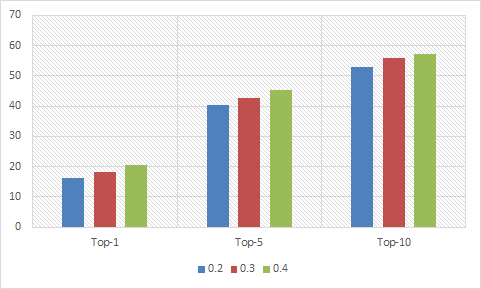
\includegraphics[scale=0.80]{Performance-rvsm+simi+co}
	\caption{The impact of $\alpha$ on bug localization performance (Top-1, Top-5, Top-10)}.
	\label{fig:PerformanceTopK}
\end{figure}


%\begin{figure}
%	\centering
%	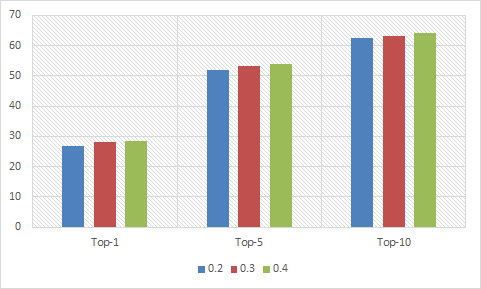
\includegraphics[scale=0.80]{Performance-vsm+co}
%	\caption{The impact of $\alpha$ on bug localization performance (Top-1, Top-5, Top-10)} for proposed approach2.
%	\label{fig:PerformanceTopK2}
%	\end{figure}

\begin{figure}
	\centering
	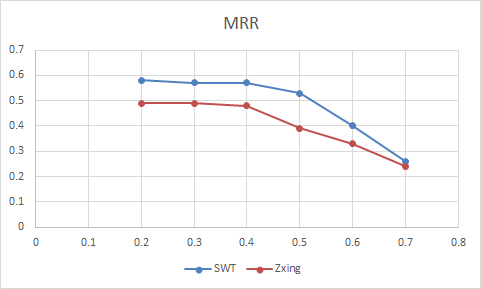
\includegraphics[scale=0.80]{MRR-SWT-Zxing}
	\caption{The impact of $\alpha$ on bug localization performance (MRR)}
	\label{fig:MRR}
\end{figure}

\begin{figure}
	\centering
	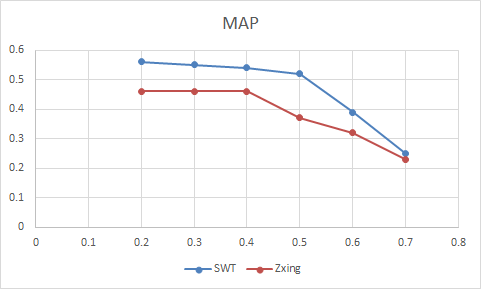
\includegraphics[scale=0.80]{MAP-SWT-Zxing}
	\caption{The impact of $\alpha$ on bug localization performance (MAP)}
	\label{fig:MAP}
\end{figure}
%\subsection{Impact of varying the value of alpha on BLuAMIR in terms of MAP and MRR}

We evaluate the impact of association score
on bug localization performance, with different $\alpha$ values in terms of MAP@10 and MRR@10 for SWT and Zxing datasets. At the beginning, the bug localization performance increases when the $\alpha$ value increases. However, after a certain point, further increase of the $alpha$ value will decrease the performance. For example, Figure \ref{fig:MRR} and \ref{fig:MAP} show the bug localization performance (measured in terms of MRR@10 and MAP@10) for the SWT and Zxing projects. When the $\alpha$ value increases from 0.1 to 0.4, both MRR and MAP values increases consistently. Increasing $\alpha$ value further from 0.4 to 0.7 however leads to lower performance. Note that we obtain the best bug localization performance when $\alpha$ is between 0.3 and 0.4. As association score is based on the association map between keywords and their associated source files, thus no direct matching of vocabulary is required. Therefore, the results obtained from the impact of $\alpha$ on bug localization performance (i.e., Hit@k, MRR@10 and MAP@10) also suggest that in the case of vocabulary missmatch issue, our association score can assist to improve the retrieval performance. This also answers RQ2.





%We combine co-occurence rank with VSM score in Approach1 and rVSM and Simi scores in Approach2. We apply both of these approaches on Eclipse dataset. We also replicate baseline techniques for those results, which are provided in Table \ref{tab:Performance1} and Table \ref{tab:Performance2}. Here, we can see that both cases BLuAMIR outperforms in terms of Top-1, Top-5, Top-10, MRR and MAP. 




\textbf{Answering RQ3:} \label{answerRQ3}
We investigate how large files problem is eliminated in BLuAMIR. First we perform a query-wise ranking comparison between baseline basic VSM and BLuAMIR on Eclipse dataset. The results are shown in Table \ref{tab:Query-Rank}.
BLuAMIR improves 41.05\% with having a mean of 13 and worsen 19.37\% with a mean of 38.10 over baseline VSM. 

\begin{table*}[htbp]
	\centering
	\caption{Query-wise Rank Comparison on Eclipse Dataset}
	\label{tab:Query-Rank}
	%\resizebox{3.4in}{!}{%
	\begin{tabular}{c|c||c|c|c||c|c|c|c|c|c}
		\hline
		%\begin{tabular}[c]{@{}c@{}}\#Bugs for \\ developing \\ map databases\end{tabular} &
		%			\begin{tabular}[c]{@{}c@{}} \textit{alpha} \end{tabular} & \begin{tabular}[c]{@{}c@{}}Bug\\Localization \\ Technique\end{tabular} & \begin{tabular}[c]{@{}c@{}}Top 1\\ \%\end{tabular} & 
		%			\begin{tabular}[c]{@{}c@{}}Top 5\\ \%\end{tabular} & 
		%			\begin{tabular}[c]{@{}c@{}}Top 10\\ \%\end{tabular} &
		%			\begin{tabular}[c]{@{}c@{}} MRR \end{tabular} & 
		%			\begin{tabular}[c]{@{}c@{}} MAP \end{tabular} \\
		
		\textbf{Technique}
		& \textbf{Total}
		& \textbf{\#Improved}
		& \textbf{Mean}
		& \textbf{Min.} 
		& \textbf{Max.} & 
		\textbf{\#Worsened} &
		\textbf{Mean}  & 
		\textbf{Min.} &
		\textbf{Max.} &
		\textbf{\# Preserved}  \\
		\hline \hline
		BugLocator & 
		3075 &
	 &
	 &
	 &
		 &
	 &
	 &
	 &
		 &
		\\ \hline
		BLUiR & 
		3075 &
		&
		&
		&
		&
		&
		&
		&
		&
		\\ \hline
		BLuAMIR & 
		3072 &
		1261 (41.05\%) &
		13 &
		1 &
		88 &
		595 (19.37\%) &
		38.10 &
		1 &
		917 &
		1216 (39.58\%)\\
		\hline
	\end{tabular}
	\centering
\end{table*}

Therefore, it is proven that BLuAMIR is showing improvement over baseline VSM and hence, we select a collection of Eclipse queries for a depth analysis.
Second, we perform a query wise ranking comparison for BLuAMIR on 30 queries from Eclipse system, which is given in Figure \ref{fig:RankImprovement}. Here, X-axis represents query number and Y-axis represents the difference of best rank retried by VSM annd our proposed BLuAMIR. Among 25 query, 10 cases BLuAMIR performs better than VSM, 6 cases VSM retrieves better ranked results than BLuAMIR and 9 cases they both do the same raking retrieval. As most cases BLuMIR provides better ranked results, we closely investigate the ranked results for several bugs. 
%\begin{figure}
%	\centering
%	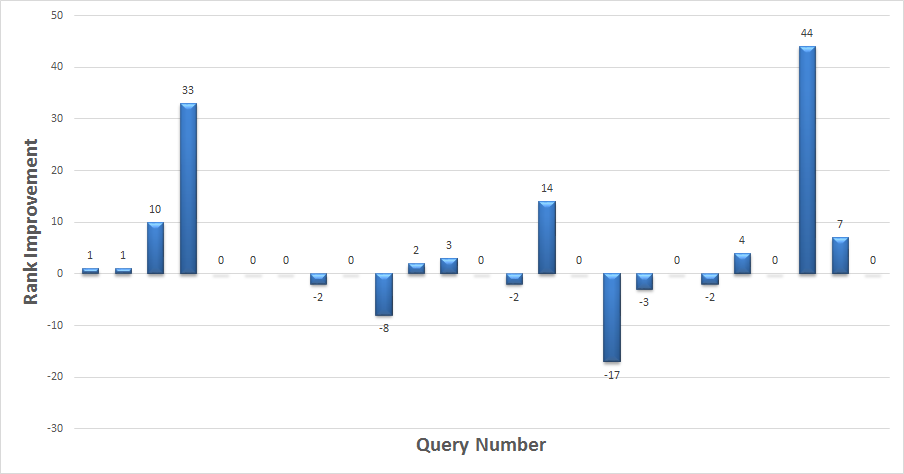
\includegraphics[scale=0.45]{RankImprovement}
%	\caption{Quey wise comparison between baseline VSM and BLuAMIR for 30 Eclipse Query}
%	\label{fig:RankImprovement}
%\end{figure}

\textbf{case \#1} Consider bug \#95561. The title of this bug is \textit{[Perspectives] Workbench flashes when synchronizing}. We have found 1 source code file (i.e., org.eclipse.ui.internal.WorkbenchPage.java) in rank \#2 from the obtained results collected from BLuAMIR. No gold set files are resulted from VSM technique in Hit@10. 
However, this source code file is obtained as rank \#30, \#26, and \#4 in the ranked results collected by applying BugLocator\cite{Jian}, basic VSM, and BLUiR\cite{Saha} respectively. 
So, we go deeper into ranking score level. The VSM score for this file is 0.45, which is lower than other smaller files. 
Because of the length of this file is too large (i.e., contains more than 14K words) making the VSM score too low. On the other hand, in BLuAMIR, this file has association score 0f 0.95, which make total score of 0.65 (i.e., 0.95*0.40+0.45*0.60), put this on rank \#2. From this case study, it is clear that association mapping between fixed bug report keywords into their corresponding source files can overcome the noise associated with large files. Even if the query and recommended buggy files do not share same keyword but previously shared same concept can aid locating that query. 
We also noted that the ground truth associated with bug \#95561 contains three large files (i.e., Workbench.java, WorkbenchPage.java, and WorkbenchWindow.java), and all of them are too large (i.e., having sizes 26 KB, 41 KB and 32KB) to retrieve by any VSM-based technique. Note of them are retrieved by VSM technique in Hit@10. Therefore, this kind of large files problem can be successfully eliminated by our proposed association score.

%***Find some queries having vocabulary miss-match problem

%\textbf{Answering RQ4:}
%We compare the performance of BLuAMIR with state-of-the-art bug localization technique, BugLocator proposed by \citet{Jian} on two dataset i.e., SWT and Zxing. These results can be found in Table \ref{tab:performance3}. For SWT, we can see our tool BLuAMIR performs better for Top-1, Top-5, MRR and MAP. However, for Top-10 BLuAmir is comparable with Buglocator. On the other hand, for Zxing our tool BLuAMIR outperforms for top-5, top-10 and MAP. So we can say that our proposed tool BLuAMIR outperforms most cases and comparable for a few cases with state-of-the-art bug localization technique.

\section{Threats To Validity}\label{sec:threats}
This section discusses the validity and generalizability of our findings. In particular, we discuss Construct Validity, Internal Validity, and External Validity.

\textbf{Internal Validity:} We used three artifacts of a software repository: bug Reports, source codes and version logs, which are generally well understood. Our evaluation uses four dataset - all of them collected from the same benchmark dataset of bug reports and source code shared by \citet{Jian}. Bug reports provide crucial information for developers to fix the bugs. A “bad” bug report could cause a delay in bug fixing. Our proposed approach also relies on the quality of bug reports. If a bug report does not provide enough information, or provides misleading information, the performance of BLuAMIR is adversely affected.

\textbf{External Validity:} 
The nature of the data in open source projects may be different from those in projects developed by well-managed software organizations. We need to evaluate if our solution can be directly applied to commercial projects. We leave this as a future work. Then we will perform statistical tests to show that the improvement of our approach is statistically significant.

\textbf{Construct Validity}
In our experiment, we use three evaluation metrics, i.e., Hit@k rank, MAP and MRR, and one statistical test, i.e., Wilcoxon signed-rank test. These metrics have been widely used before to evaluate previous approaches \cite{Jian, Saha} and are well- known IR metrics. Thus, we argue that our research has strong construct validity.

\textbf{Reliability:}
In our experiment section, we performed numerous experiments using various combinations of weighting functions to find the optimum parameters and the best accuracy of bug localization. The optimized $\alpha$ values are based on our experiments and are only for our proposed tool BLuAMIR. To automatically optimize control parameters for target projects, in the future we will expand our proposed approach using machine learning methods or generic algorithms.

\section{Related Work}\label{relatedwork}
There are many bug localization approaches proposed so far. They can be broadly categorized into two types - dynamic and static techniques. Generally, dynamic approaches can localize a bug much more precisely than static approaches. These techniques usually contrast the program spectra information (such as execution statistics) between passed and failed executions to compute the fault suspiciousness of individual program elements (such as statements, branches, and predicates), and rank these program elements by their fault suspiciousness. Developers may then locate faults by examining a list of program elements sorted by their suspiciousness. Some of the well known dynamic approaches are spectrum-based fault localization, e.g., \cite{Abreu,Jones,Lucia,SahaFault}, model-based fault localization, e.g., \cite{Feldman,Mayer}, dynamic slicing \cite{Zhang:2005}, delta debugging \cite{Zeller:2002}. 

Static approaches, on the other hand, do not require any program test cases or execution traces. In most cases, they need only program source code and bug reports. They are also computationally efficient. The static approaches usually can be categorized into two groups: program analysis based approaches and IR-based approaches. FindBugs is a program analysis based approach that locates a bug based on some predefined bug patterns \cite{FindBug}. Therefore, FindBug does not even need a bug report. However, it often detects too many false positives and misses many real bugs \cite{Tang}. IR-based approaches use information retrieval techniques (such as, TFIDF, LSA, LDA, etc.) to calculate the similarity between a bug report and a source code file. There are three traditionally-dominant IR paradigms TF.IDF \cite{Salton}, the “probabilistic approach” known as BM25 \cite{Robertson}, or more recent language modeling \cite{Ponte}. Another empirical study \cite{Fang} show that all three approaches perform comparably when well-tuned. However, \citet{Rao} investigates many standard information retrieval techniques for bug localization and find that simpler techniques, e.g., TFIDF and SUM, perform the best. 

In contrast with shallow “bag-of-words” models, latent semantic indexing (LSI) induces latent concepts. While a probabilistic variant of LSI has been devised \cite{Hofmann}, its probability model was found to be deficient.
%On the other hand, \citet{Lukins} created a Latent Dirichlet Allocation (LDA) model from the source code which provided word-topic modeling and topic-document distribution.
\citet{Lukins2} use Latent Dirichlet Allocation (LDA), which is a well-known topic modeling approach, to localize bug \cite{Lukins2}.
However, LSI is rarely used in practice today due to errors in induced concepts introducing more harm than good \cite{Hofmann} and LDA is not be able to predict the appropriate topic because it followed a generative topic model in a probabilistic way \cite{Lukins}.

\citet{Sisman} propose a history-aware IR-based bug localization solution to achieve a better
result. \citet{Jian} propose BugLocator, which leverages similarities among bug reports and uses refined vector space model to perform bug localization. \citet{Saha} build BLUiR that consider the structure of bug reports and source code files and employ structured retrieval to achieve a better result. \citet{Moreno} uses a text retrieval based technique and stack trace analysis to perform bug localization. To locate buggy files, they combines the textual similarity between a bug report and a code unit and the structural similarity between the stack trace and the code unit. Different from the existing IR-based bug localization approaches, \citet{Wang} propose AmaLgam, a new method for locating relevant buggy files that put together version history, similar report, and structure, to achieve better performance. Later \cite{Wang2} also propose AmaLgam+, which is a method for locating relevant buggy files that puts together fives sources of information i.e., version history, similar reports, structure, stack traces, and reporter information.
In our proposed technique BLuAMIR, we use three sources of information i.e., bug reports, source codes and version history.






\section{Conclusion and Future Work} \label{sec:conclusionANDfuture}
During software evolution of a system, a large number of bug reports are submitted. For a large software project, developers must may need to examine a large number of source code files in order to locate the buggy files responsible for a bug, which is a tedious and expensive work. In this paper, we propose BLuAMIR, a new bug localization technique not only based on lexical similarity but also an implicit association map between bug report keywords with their associated source codes. We perform a large-scale experiments on four projects, namely Eclipse, SWT, AspectJ and ZXing to localize more than 3,000 bugs. Our experiment of those dataset show that on average our technique can locate buggy files with a Top-10 accuracy of 74.06\% and a mean reciprocal rank@10 of 0.52 and a mean precision average@10 of 41\%, which are highly promising. We also compare our technique with three state-of-the-art IR-based bug localization techniques i.e., BugScout\cite{Nguyen}, BugLocator\cite{Jian} and BLUiR\cite{Saha}.  This also confirms superiority of our technique. Our technique can localize bugs with 6\%--54\% higher accuracy (i.e., Hit@5), 4\%--32\% higher precision (i.e., MAP) and 8\%--27\% higher reciprocal ranks (i.e., MRR) than these state-of-the-art approaches. This also confirms superiority of our proposed bug localization approach. 

In the future, we will explore if several other bug related information such as bug report structure, source code structure, stack traces, reporter information, similar bug information can be integrated into our approach in order to improve bug localization performance. We would also like to reduce the threats to external validity further by applying our approach on more bug reports collected from other software systems.

\bibliographystyle{plainnat}
\scriptsize
\bibliography{test}
%\begin{thebibliography}{00}
%\bibitem{b1} G. Eason, B. Noble, and I. N. Sneddon, ``On certain integrals of Lipschitz-Hankel type involving products of Bessel functions,'' Phil. Trans. Roy. Soc. London, vol. A247, pp. 529--551, April 1955.
%\bibitem{b2} J. Clerk Maxwell, A Treatise on Electricity and Magnetism, 3rd ed., vol. 2. Oxford: Clarendon, 1892, pp.68--73.
%\bibitem{b3} I. S. Jacobs and C. P. Bean, ``Fine particles, thin films and exchange anisotropy,'' in Magnetism, vol. III, G. T. Rado and H. Suhl, Eds. New York: Academic, 1963, pp. 271--350.
%\bibitem{b4} K. Elissa, ``Title of paper if known,'' unpublished.
%\bibitem{b5} R. Nicole, ``Title of paper with only first word capitalized,'' J. Name Stand. Abbrev., in press.
%\bibitem{b6} Y. Yorozu, M. Hirano, K. Oka, and Y. Tagawa, ``Electron spectroscopy studies on magneto-optical media and plastic substrate interface,'' IEEE Transl. J. Magn. Japan, vol. 2, pp. 740--741, August 1987 [Digests 9th Annual Conf. Magnetics Japan, p. 301, 1982].
%\bibitem{b7} M. Young, The Technical Writer's Handbook. Mill Valley, CA: University Science, 1989.
%\end{thebibliography}



\end{document}
